\documentclass[journal]{IEEEtran}
\IEEEoverridecommandlockouts
% The preceding line is only needed to identify funding in the first footnote. If that is unneeded, please comment it out.
\usepackage{cite}
\usepackage{amsmath,amssymb,amsfonts}
\usepackage{algorithmic}
\usepackage{graphicx}
\usepackage{textcomp}
\usepackage{xcolor}
\def\BibTeX{{\rm B\kern-.05em{\sc i\kern-.025em b}\kern-.08em
    T\kern-.1667em\lower.7ex\hbox{E}\kern-.125emX}}

\usepackage{graphicx,url}
\usepackage[raggedright]{subfigure}
\usepackage[none]{hyphenat}
\usepackage{amsmath,amsfonts}
\usepackage{cite}
\usepackage[brazil]{babel}

\sloppy
\usepackage{placeins}
\usepackage{url}
\usepackage{threeparttable}
\usepackage{comment}


%\makeatletter
%\renewcommand{\fnum@figure}{Figura \thefigure}
%\makeatother

\def\IEEEkeywordsname{Index Terms}


    
   
    
    
\begin{document}

\title{Modelagem Estocástica do Consumo de Energia Elétrica em Estados Norte-Americanos}
%\thanks{Este trabalho foi realizado com apoio da Coordenação de Aperfeiçoamento de Pessoal de Nível Superior - Brasil (CAPES) - Código de Financiamento 001.}

\author{Everton Costa Santos

\thanks{O autor Everton Costa Santos é da Universidade Federal de Juiz de Fora (UFJF), Juiz de Fora, MG, Brazil. E-mail: everton.santos@estudante.ufjf.br.}

%\thanks{
%Este trabalho foi realizado com apoio da Coordenação de Aperfeiçoamento de Pessoal de Nível Superior - Brasil (CAPES) - Código de Financiamento 001.}
}



\markboth{IEEE Latin America Transactions}%
{}


\maketitle

\begin{abstract}

Este trabalho apresenta um estudo de modelagem estocástica do consumo de energia elétrica em estados norte-americanos atendidos pela PJM Interconnection LLC. Utilizou-se um conjunto de dados públicos obtido na plataforma Kaggle, abrangendo medições horárias. O estudo foi conduzido em duas etapas: (i) modelagem assumindo independência e distribuição idêntica (i.i.d), com análise exploratória, ajuste de distribuições e teste de Kolmogorov–Smirnov; e (ii) modelagem baseada em séries temporais com o modelo ARIMA, incluindo testes de estacionariedade e análise de resíduos. Os resultados indicam que o ARIMA(1,1,1) apresentou bom desempenho para previsões in-sample e em período posterior (MAPE de 1,42\% em nov. 2017), embora ainda apresente autocorrelação nos resíduos


\end{abstract}

%\begin{IEEEkeywords}
%component, formatting, style, styling, insert
%\end{IEEEkeywords}

\begin{IEEEkeywords}
Modelagem Estocástica, Consumo de Energia, ARIMA, Séries Temporais.
\end{IEEEkeywords}


\section{Introdução}
\label{sec_Intro}

%\IEEEPARstart{D}e acordo com a GSMA \emph{Intelligence} \cite{gsma2017}, este parágrafo deve ser utilizado para motivar o leitor sobre o problema.

%Este parágrafo serve para detalhar mais o problema, incluindo ctações de livros \cite{parsons2000}, artigos de survey ou tutoriais \cite{stephens1970}. Tal detalhamento pode precisar de mais 1 ou 2 parágrafos.

%Neste parágrafo é feita uma revisão bibliográfica rápida sobre o problema, mostrando como alguns autores abordam o problema. Aqui são citados artigos e mais específicos, principalmente os que se deseja comparar \cite{parsons2000,patzold,yacoub1999,chetan}.

%Neste parágrafo apresenta-se os objetivos do trabalho e a importância dele, mostrando os seu diferencial com relação aos artigos citados. É descrito também de forma rápida a metodologia utilizada e os resultados. Pode ocupar mais de um parágrafo.

%Este parágrafo apresenta a estrutura do artigo. Este artigo está dividido como a seguir. Na Seção~\ref{prototipo} são apresentados os materiais e métodos usados na  investigação. A apresentação e discussão dos resultados estão expostos na Seção~\ref{sec_results}. Finalmente, a Seção~\ref{sec_conclusoes} traz as considerações finais do trabalho.


\IEEEPARstart{A} energia elétrica trata-se de um insumo fundamental para a dinâmica de uma sociedade, e a aplicações de métodos estatísticos são de grande valia para o seu gerenciamento\cite{marcos2021}. 

A previsão do consumo de energia elétrica é crucial para o planejamento da expansão da oferta, a operação segura do sistema e a formulação de políticas públicas. Evidências empíricas mostram que o crescimento econômico e a evolução tecnológica se associam à elevação da demanda, reforçando a necessidade de modelos de previsão transparentes e acurados. No Brasil, abordagens clássicas de séries temporais têm sido eficazes: modelos ARIMA sazonais, combinados a uma estratégia hierárquica \textit{bottom-up}, geraram previsões consistentes para o setor industrial por regiões \cite{filho2025}; além disso, comparações entre ARIMA e estruturas multivariadas VAR--VEC indicam que, embora ARIMA apresente bom desempenho geral, modelos multivariados podem ganhar vantagem no curtíssimo prazo quando incorporam variáveis explicativas como PIB e tarifas \cite{nunes2022}. Mais recentemente, estudos apontam ganhos ao combinar ARIMA com redes neurais recorrentes (LSTM) para capturar não linearidades e tendências de mais longo prazo, com ganhos de acurácia em janelas operacionais relevantes \cite{goncalves2025}.

No cenário internacional, métodos híbridos e comparativos reforçam essa complementariedade. Um modelo híbrido SARIMA--neurônio simples multiplicativo foi proposto para capturar simultaneamente componentes lineares e não lineares em séries de consumo mensal de eletricidade, mostrando superioridade frente a especificações isoladas \cite{velasquez2013}. Em aplicações de \textit{smart grids} com medições em alta frequência, análises comparativas entre ARIMA, SARIMA e LSTM indicam vantagem do LSTM em métricas de erro, sem dispensar o valor dos modelos estocásticos pela interpretabilidade e pela diagnose rigorosa de resíduos \cite{dubey2021}. À luz dessas evidências, este artigo adota a modelagem estocástica (com ênfase no modelo ARIMA) para investigar o consumo de energia elétrica em estados norte-americanos, buscando mostrar a aplicabilidade em casos reais e sua eficácia. A base de dados foi obtida em \cite{Kaggle2025}, a qual refere-se ao consumo de energia elétrica de uma região gerenciada pela a PJM Interconnection LLC. 

A motivação para este estudo reside na importância de prever adequadamente o consumo de energia, proporcionando melhorias na gestão, permitindo melhor alocação de recursos, redução de custos, maior confiabilidade de sistemas e, por fim, é uma lógica que pode ser aplicada em diversos cenários de outros países, desde que se tenha um conjunto apropriado de dados. Para isto o modelo ARIMA foi testado, em função das características da variável.

O ARIMA \emph{(AutoRegressive   Integrated Moving Average)} trata-se de uma classe de métodos estatísticos que busca realizar previsões de séries temporais. É uma   generalização   de   um   modelo   mais   simples chamado  ARMA \emph{(AutoRegressive Moving  Average)}\cite{ynoguti2012} \cite{leon2008}.


Sendo assim, o objetivo deste trabalho é entender as caractísticas dos dados por meio de uma modelagem típica para dados i.i.d e, posteriormente, uma modelagem considerando os mesmos como um processo estocástico, por meio do método supracitado, ARIMA.

Este artigo está organizado da seguinte forma: na Seção II são apresentados os materiais e métodos. A Seção III traz os resultados e discussões. Por fim, a Seção IV apresenta as conclusões.



%\section{Materiais e Métodos}
%\label{prototipo}

%Esta Seção é dividida em três partes, apresentando os seguintes conteúdos: (A) descrição do \emph{setup} de medições incluindo a metodologia utilizada para as coletas de dados; %encontram-se na Seção~\ref{sec_setup}; 
%(B) análise do sinal e métodos estatísticos utilizados para processar os dados ;% são apresentados na Seção~\ref{sec_estimacao}; 
%(C) seção adicional, caso necessário.

%\subsection{Setup de Medição}
%\label{sec_setup}

%Esta Seção é usada para descrição dos procedimentos e equipamentos usados na medição. Ela pode conter vários parágrafos e figuras, como por exemplo a Figura~\ref{fig:d_fita}

%
%\begin{figure}[ht]
%   \centering
%    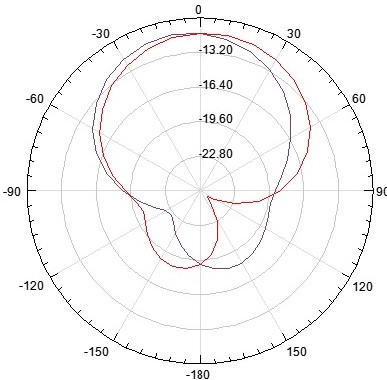
\includegraphics[height=0.5\columnwidth]{d_fita}
%    \label{fig:d_fita}
%    \caption{Exemplo de Figura.}
%\end{figure}
%

%\subsection{Processamento das Amostras e Estimação de Parâmetros}
%\label{sec_estimacao}


%Esta Seção é usada para descrição dos procedimentos e equipamentos usados na medição. Ela pode conter vários parágrafos, figuras, tabelas e equações. 

%A equação deve fazer parte do texto, portanto ela deve ser pontuada e só referenciada após aparecer no texto. Por exemplo, um método de filtragem muito utilizado é o algoritmo de janela móvel~\cite{hermano2008}, que recebe como entrada o tamanho da janela a ser utilizada (2$L$ + 1) e retorna um vetor em que cada ponto~$\hat{x_i}$ é a média calculada entre ele mesmo, os próximos $L$ pontos e os $L$ pontos anteriores, isto é,
%
%\begin{equation}
%    \hat{x_i} = \frac{1}{2L + 1} \sum_{n = i - L}^{i + L} x_n.
%    \label{eq:eq-slicewin}
%\end{equation}

%Outro exemplo de equação é mostrado a seguir. O sinal recebido $s(t)$ é dado por
%
%\begin{equation}
%    s(t) = l(t) + p(t),
%    \label{eq:eq-signal}
%\end{equation}
%
%\noindent em que $l(t)$ é o ruído de baixa potência e $p(t)$ é o sinal transmitido.
%


%Baseado em \eqref{eq:eq-signal}, é possível gerar um sinal de referência como mostrado na Figura \ref{fig:parametro_M}.
%
%\begin{figure}[!htb]
%    \centering
%    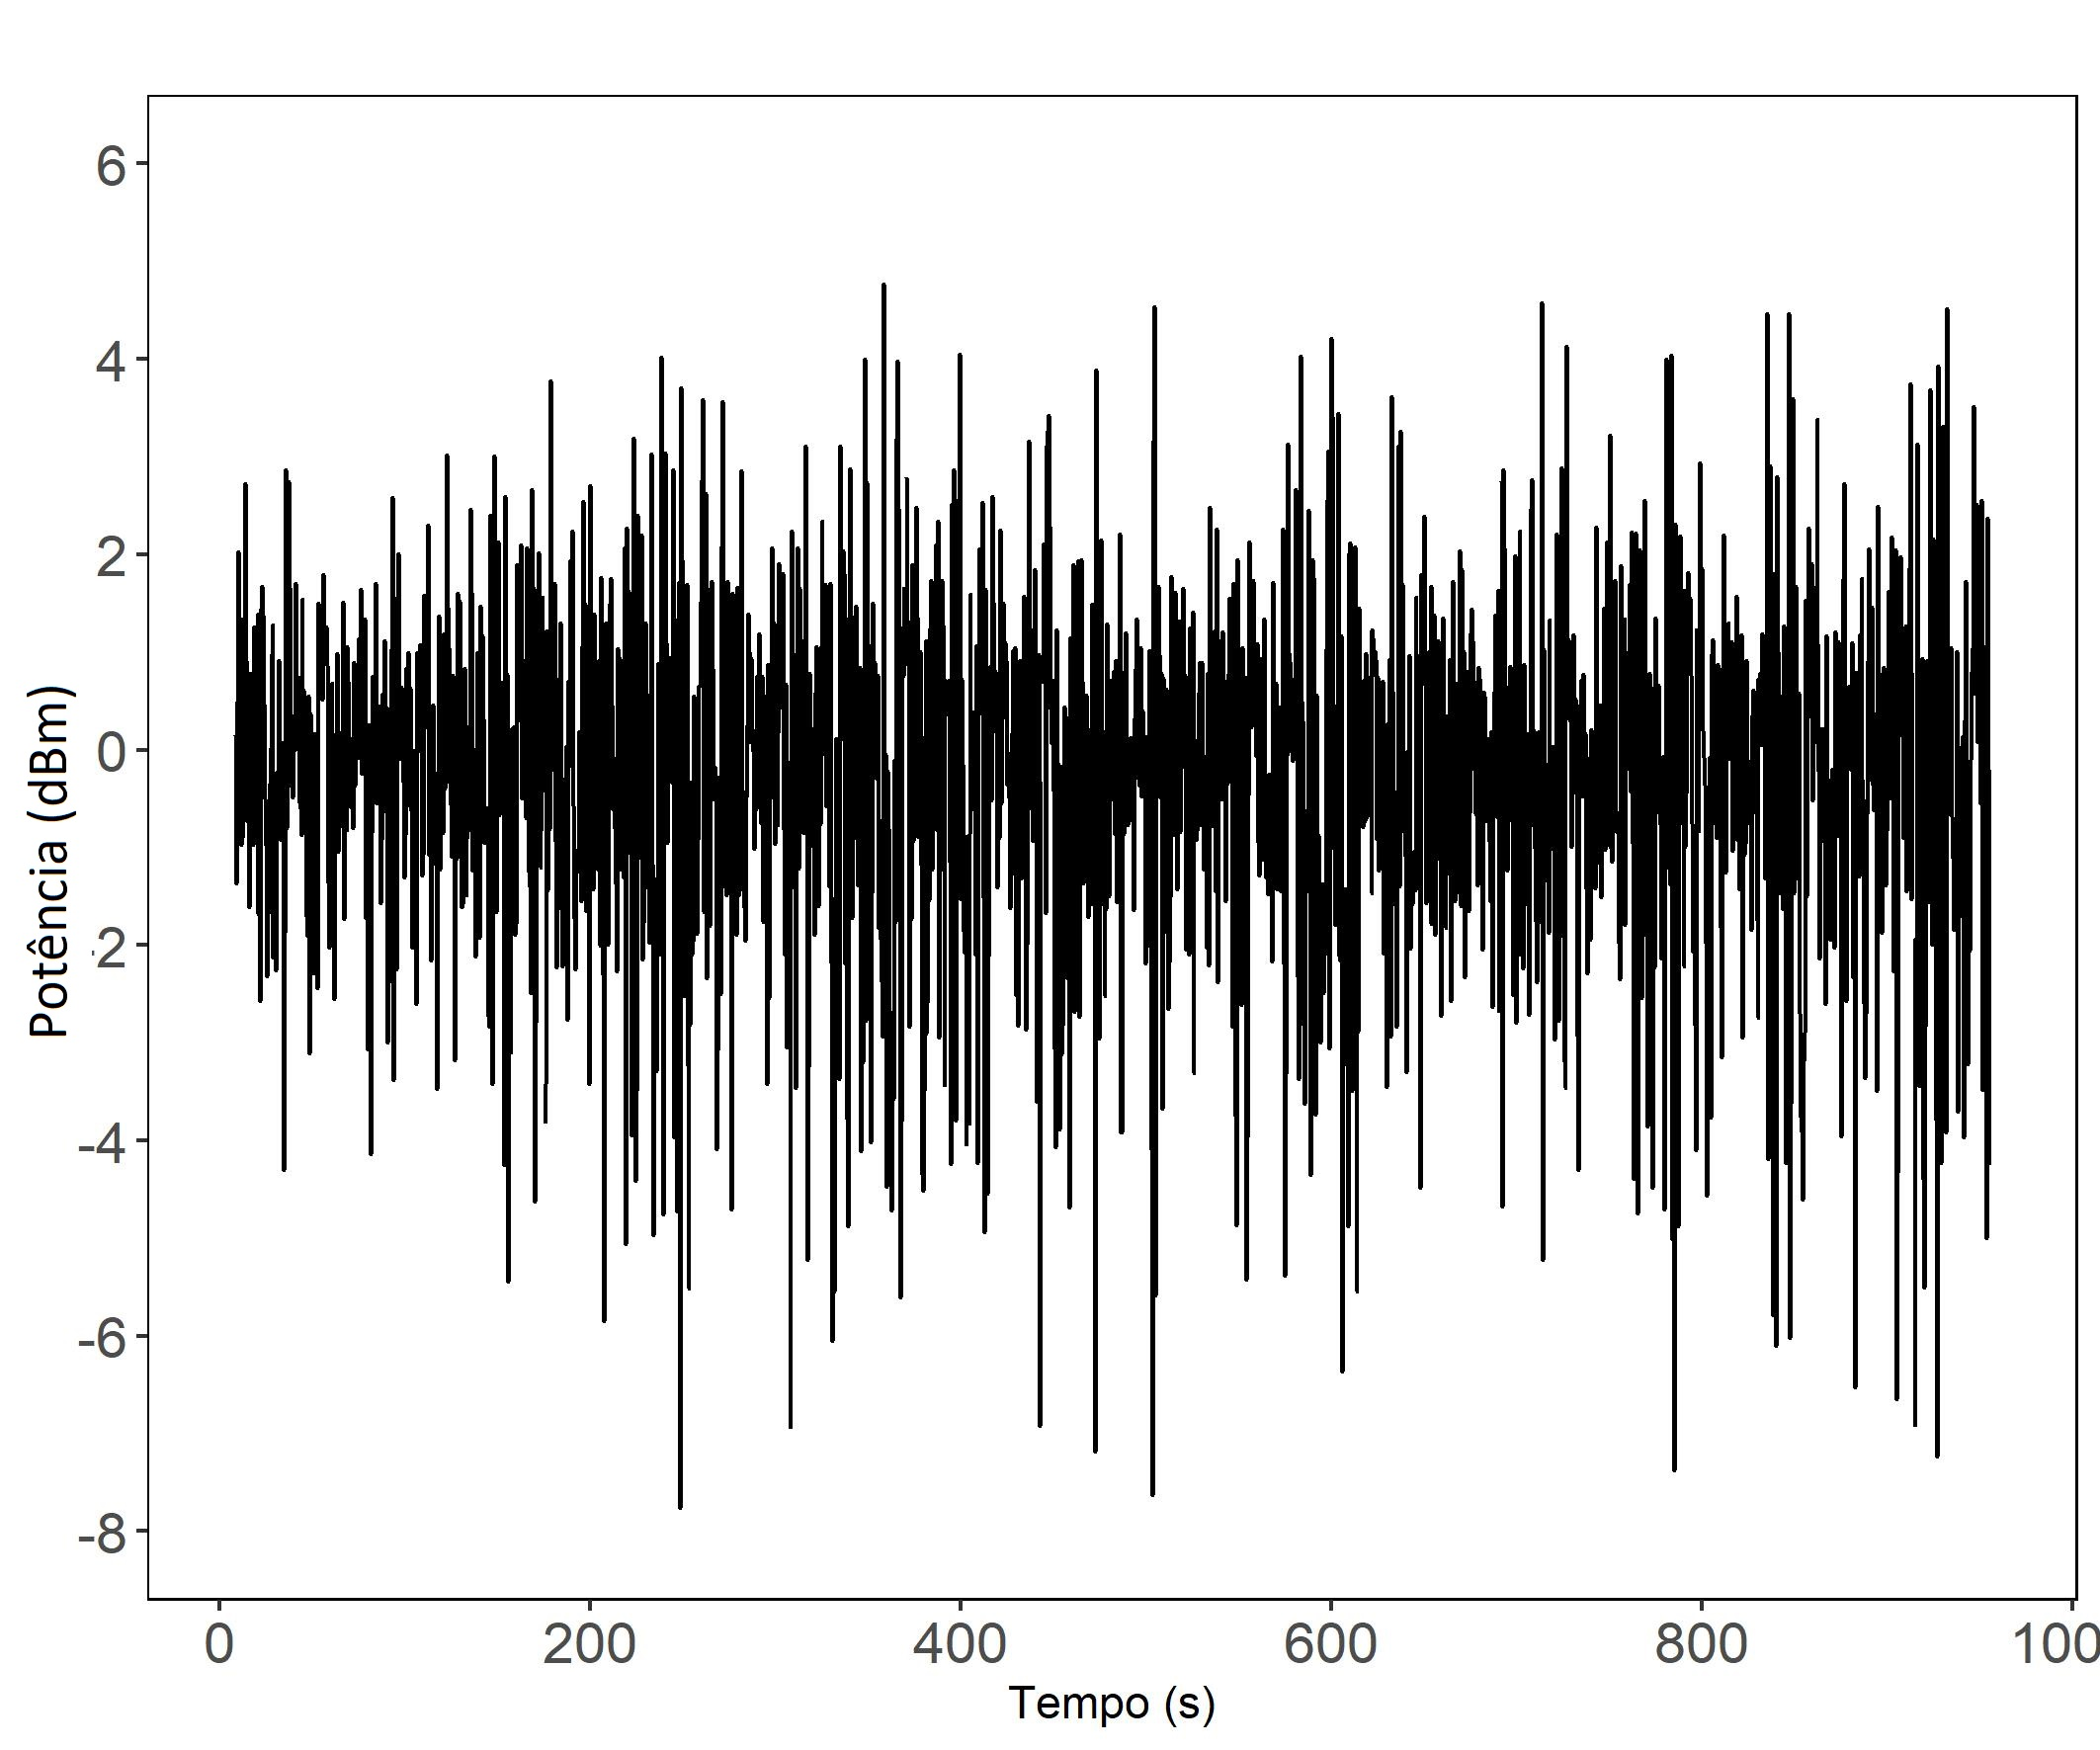
\includegraphics[height=0.65\columnwidth]{dia2alto.jpeg}
%    \label{fig:parametro_M}
%    \caption{Exemplo de Figura de sinal.}
%\end{figure}


\section{Materiais e Métodos}
\label{prototipo}
\subsection {Base de Dados} 
O conjunto de dados foi obtido por meio da plataforma Kaggle, contendo os registros de consumo total de energia (MW) por hora de 2005 a 2017, considerando a região operada pela PJM Interconnection LLC. O citado banco de dados é formado por uma amostra de tamanho 113931\cite{Kaggle2025}.

\subsection {Metodologia i.i.d.}
Buscando comprender o grau de independência dos dados, escolheu-se uma amostra que, hipoteticamente, atenderia critérios para a modelagem dos dados como sendo identicamente indepentendes. A escolha foi o consumo de energia elétrica, às 4h durante cada mês de março de cada um dos 13 anos.

Após a seleção da amostra, foram seguidas as etapas básicas da modelagem sugeridas por \cite{chwif2010}:

1. Cálculo de medidas de posição, dispersão e assimetria;

2. Análise de \emph{outlier};

3. Construção de histogramas e avaliação de distribuições candidatas;

4. Aplicação do teste de Kolmogorov–Smirnov;

5. Verificação da independência dos dados pelo teste de Ljung–Box.

Dentro destas etapas citadas nesta seção, vale destacar a aplicação do gráfico \emph{Box Plot} modificado, o qual consiste em construir um intervalo de valores a partir dos quartis da amostra. Se considerarmos que Q1 e Q3 são, respectivamente, os valores do
 primeiro e terceiro quartis, a amplitude interquartil, A, é calculada pela diferença que segue:

 \begin{equation}
    A = Q3 - Q1
    \label{eq:eq-signal}
\end{equation}

Considera-se um valor discrepante ou \emph{outlier} moderado qualquer valor que estiver abaixo de Q1 – 1,5A ou acima de Q3 + 1,5A. De modo semelhante, considera-se um valor discrepante ou \emph{outlier} extremo, qualquer valor que estiver abaixo de Q1 – 3A ou acima de Q3 + 3A\cite{chwif2010}.

Outro destaque necessário nesta seção é o Teste de Ljung--Box. O teste de Ljung--Box é amplamente utilizado na análise de séries temporais para verificar 
se os resíduos de um modelo ajustado podem ser considerados \textit{ruído branco}. 
Em termos práticos, o teste avalia se existe autocorrelação significativa em diferentes 
defasagens (\textit{lags}) da série residual. A presença de autocorrelação indicaria 
que o modelo não capturou toda a estrutura temporal dos dados, comprometendo a validade 
das inferências e previsões.

A hipótese nula do teste é formulada como:
\[
H_0 : \rho_1 = \rho_2 = \dots = \rho_h = 0,
\]

em que $\rho_k$ representa o coeficiente de autocorrelação da série residual na defasagem $k$, 
e $h$ é o número de defasagens consideradas no teste. Assim, $H_0$ postula que não há 
autocorrelação até a defasagem $h$, isto é, os resíduos são independentes.

O estatístico de teste proposto por Ljung e Box (1978) é dado por:
%\[
%Q = n (n+2) \sum_{k=1}^{h} \frac{\hat{\rho}_k^2}{n-k},
%\]

 \begin{equation}
    Q = n (n+2) \sum_{k=1}^{h} \frac{\hat{\rho}_k^2}{n-k},
    \label{eq:eq-signal}
\end{equation}

em que:
\begin{itemize}
    \item $n$ é o tamanho da amostra;
    \item $\hat{\rho}_k$ é a autocorrelação amostral dos resíduos na defasagem $k$;
    \item $h$ é o número de defasagens analisadas.
\end{itemize}

Sob a hipótese nula, o estatístico $Q$ segue, assintoticamente, uma distribuição 
qui-quadrado com $(h-m)$ graus de liberdade, sendo $m$ o número de parâmetros 
estimados no modelo ajustado.

A decisão do teste é baseada no valor-p: se este for menor que o nível de significância 
adotado (por exemplo, $\alpha = 0{,}05$), rejeita-se $H_0$, concluindo-se que há 
autocorrelação significativa nos resíduos até a defasagem considerada \cite{ljungbox1978}.

\subsection {Metodologia de Séries Temporais}
Após a modeagem i.i.d, buscou-se estratégias para a modelagem considerando o conjunto de dados como sendo um processo estocástico, uma vez que os mesmos referem-se ao consumo de energia elétrica, os quais variam aleatoriamente e apresentam indexação.

Sendo assim, seguindo estratégias abordadas em  \cite{nielsen2019}, as seguintes etapas foram realizadas:

1. Escolha do período de treinamento (novembro de 2016) e teste ADF para estacionariedade;

2. Aplicação de diferenciação para tornar a série estacionária;

3. Análise ACF e PACF para definição de p e q;

4. Ajuste do modelo;

5. Previsão \emph{in-sample} e \emph{out-of-sample} (novembro de 2017) para cálculo do MAPE;

6. Análise de resíduos.

As técnicas apresentadas nos passos 1 e 3 merecem um destaque, uma vez que foram cruciais para geração dos resultados. 

O teste ADF, citado no passo 1 da metodologia, é um procedimento estatístico utilizado para verificar a presença de \textit{raiz unitária} em uma série temporal, o que indicaria não-estacionariedade.
A forma geral da equação testada é:

%\[
%\Delta y_t = \alpha + \beta t + \gamma y_{t-1} + %\sum_{i=1}^{p} \delta_i \Delta y_{t-i} + \varepsilon_t,
%\]

 \begin{equation}
    \Delta y_t = \alpha + \beta t + \gamma y_{t-1} + \sum_{i=1}^{p} \delta_i \Delta y_{t-i} + \varepsilon_t,
    \label{eq:eq-signal}
\end{equation}

em que:
\begin{itemize}
    \item $y_t$ é a série temporal;
    \item $\Delta y_t = y_t - y_{t-1}$ representa a primeira diferença;
    \item $t$ é a tendência temporal determinística (opcional);
    \item $p$ é o número de defasagens adicionais incluídas para capturar autocorrelação;
    \item $\varepsilon_t$ é o termo de erro.
\end{itemize}

A hipótese nula do teste é:
\[
H_0: \gamma = 0 \quad \text{(a série possui raiz unitária, não é estacionária)},
\]
contra a alternativa
\[
H_1: \gamma < 0 \quad \text{(a série é estacionária)}.
\]


A função de autocorrelação (ACF), apresentada no passo 3, mede a dependência linear entre valores da série em diferentes defasagens.
Formalmente, para uma série $\{y_t\}$ com média $\mu$ e variância $\sigma^2$, a autocorrelação de ordem $k$ é:

%\[
%\rho_k = \frac{\mathrm{Cov}(y_t, y_{t-k})}{\sigma^2}
%= \frac{E\big[(y_t - \mu)(y_{t-k} - \mu)\big]}{E\big[(y_t - \mu)^2\big]}.
\]

 \begin{equation}
    \rho_k = \frac{\mathrm{Cov}(y_t, y_{t-k})}{\sigma^2}
= \frac{E\big[(y_t - \mu)(y_{t-k} - \mu)\big]}{E\big[(y_t - \mu)^2\big]}.
    \label{eq:eq-signal}
\end{equation}

A análise do gráfico da ACF permite identificar a presença de dependência temporal
em diferentes defasagens e auxilia na escolha da ordem do componente MA de modelos ARMA/ARIMA

Já a função de autocorrelação parcial mede a correlação entre $y_t$ e $y_{t-k}$ \textit{condicionada}
nas defasagens intermediárias $y_{t-1}, y_{t-2}, \dots, y_{t-k+1}$. Em outras palavras,
a PACF remove os efeitos indiretos de defasagens menores.

Seja $\phi_{kk}$ o coeficiente de regressão de $y_t$ em relação a $y_{t-1}, \dots, y_{t-k}$.
A PACF na defasagem $k$ é definida como:

%\[
%\phi_{kk} = \text{corr}\left(y_t - \hat{y}_t^{(1,\dots,k-1)}, \; y_{t-k} - \hat{y}_{t-k}^{(1,\dots,k-1)}\right),
\]

 \begin{equation}
\phi_{kk} = \text{corr}\left(y_t - \hat{y}_t^{(1,\dots,k-1)}, \; y_{t-k} - \hat{y}_{t-k}^{(1,\dots,k-1)}\right),
    \label{eq:eq-signal}
\end{equation}

onde $\hat{y}_t^{(1,\dots,k-1)}$ é a previsão linear de $y_t$ usando as defasagens intermediárias.
Na prática, a PACF é obtida via equações de Yule--Walker.

A análise do gráfico da PACF é utilizada para identificar a ordem do componente AR em modelos ARMA/ARIMA  \cite{nielsen2019}.

Por fim, o modelo \emph{Autoregressive Integrated Moving Average} (ARIMA) é amplamente utilizado para modelagem e previsão de séries temporais. Sua formulação geral é representada por ARIMA$(p,d,q)$, onde $p$ é a ordem autorregressiva, $d$ é o número de diferenciações aplicadas para tornar a série estacionária e $q$ é a ordem da média móvel. O modelo pode ser expresso matematicamente como:

\begin{equation}
\phi(B)(1-B)^{d} Y_{t} = \theta(B)\varepsilon_{t},
\end{equation}

em que $B$ é o operador de defasagem, $\phi(B)$ representa os coeficientes do componente autorregressivo (AR), $\theta(B)$ os coeficientes do componente de média móvel (MA) e $\varepsilon_{t}$ é o termo de erro aleatório.

Para avaliar o desempenho preditivo do modelo, uma métrica frequentemente utilizada é o Erro Percentual Quadrático Médio (MSPE, do inglês \textit{Mean Squared Percentage Error}). Esta medida penaliza desvios em termos percentuais, sendo definida como:

\begin{equation}
MSPE = \frac{1}{n} \sum_{t=1}^{n} \left( \frac{Y_{t} - \hat{Y}_{t}}{Y_{t}} \right)^{2} \times 100,
\end{equation}

onde $Y_{t}$ representa os valores observados e $\hat{Y}_{t}$ os valores previstos pelo modelo. Valores menores de $MSPE$ indicam maior precisão na previsão.




%\section{Apresentação e Discussão dos Resultados}
%\label{sec_results}

%Nesta Seção, são apresentados os resultados da medição, bem como da análise estatística do sinal. Um exemplo de calendário das medições realizadas é mostrado na Tabela~\ref{tab:medicoes}. Cada medição foi feita seguindo o procedimento descrito na Seção \ref{sec_setup}

% TABELA MEDICOES 
%\begin{table}[!htb]
 %   \centering
 %   \caption{\label{tab:medicoes} Calendário de medições.}
  %  \begin{tabular}{rrrrr}
   %     \hline\hline
    %       \textbf{Turno} & \textbf{Horário} & \textbf{Dia 1} & \textbf{Dia 2} & \textbf{Fluxo} \\
     %   \hline
      %      Manhã & 1º Intervalo & - & X & Alto \\
       %     Manhã & 2ª Aula      & - & - & Baixo\\
        %    Manhã & 2º Intervalo & - & - & Alto \\
         %   Manhã & 3º Aula      & - & X & Baixo \\
          %  Tarde & 1º Intervalo & - & - & Alto \\
           % Tarde & 2ª Aula      & X & X & Baixo\\
%            Tarde & 2º Intervalo & X & X & Alto \\
 %           Tarde & 3º Aula      & X & X & Baixo \\
  %          Noite & 1º Intervalo & X & X & Alto \\
   %     \hline\hline
%    \end{tabular}
%\end{table}


%A Figura~\ref{fig:ptrx} apresenta amostras obtidas na campanha de medição. Ela é um exemplo de como utilizar o \emph{subfigure}.

%\begin{figure}[ht]
%    \centering
    %
%    \subfigure[\label{fig:ptrx_omni_alto} Exemplo dia 1, alto fluxo.]{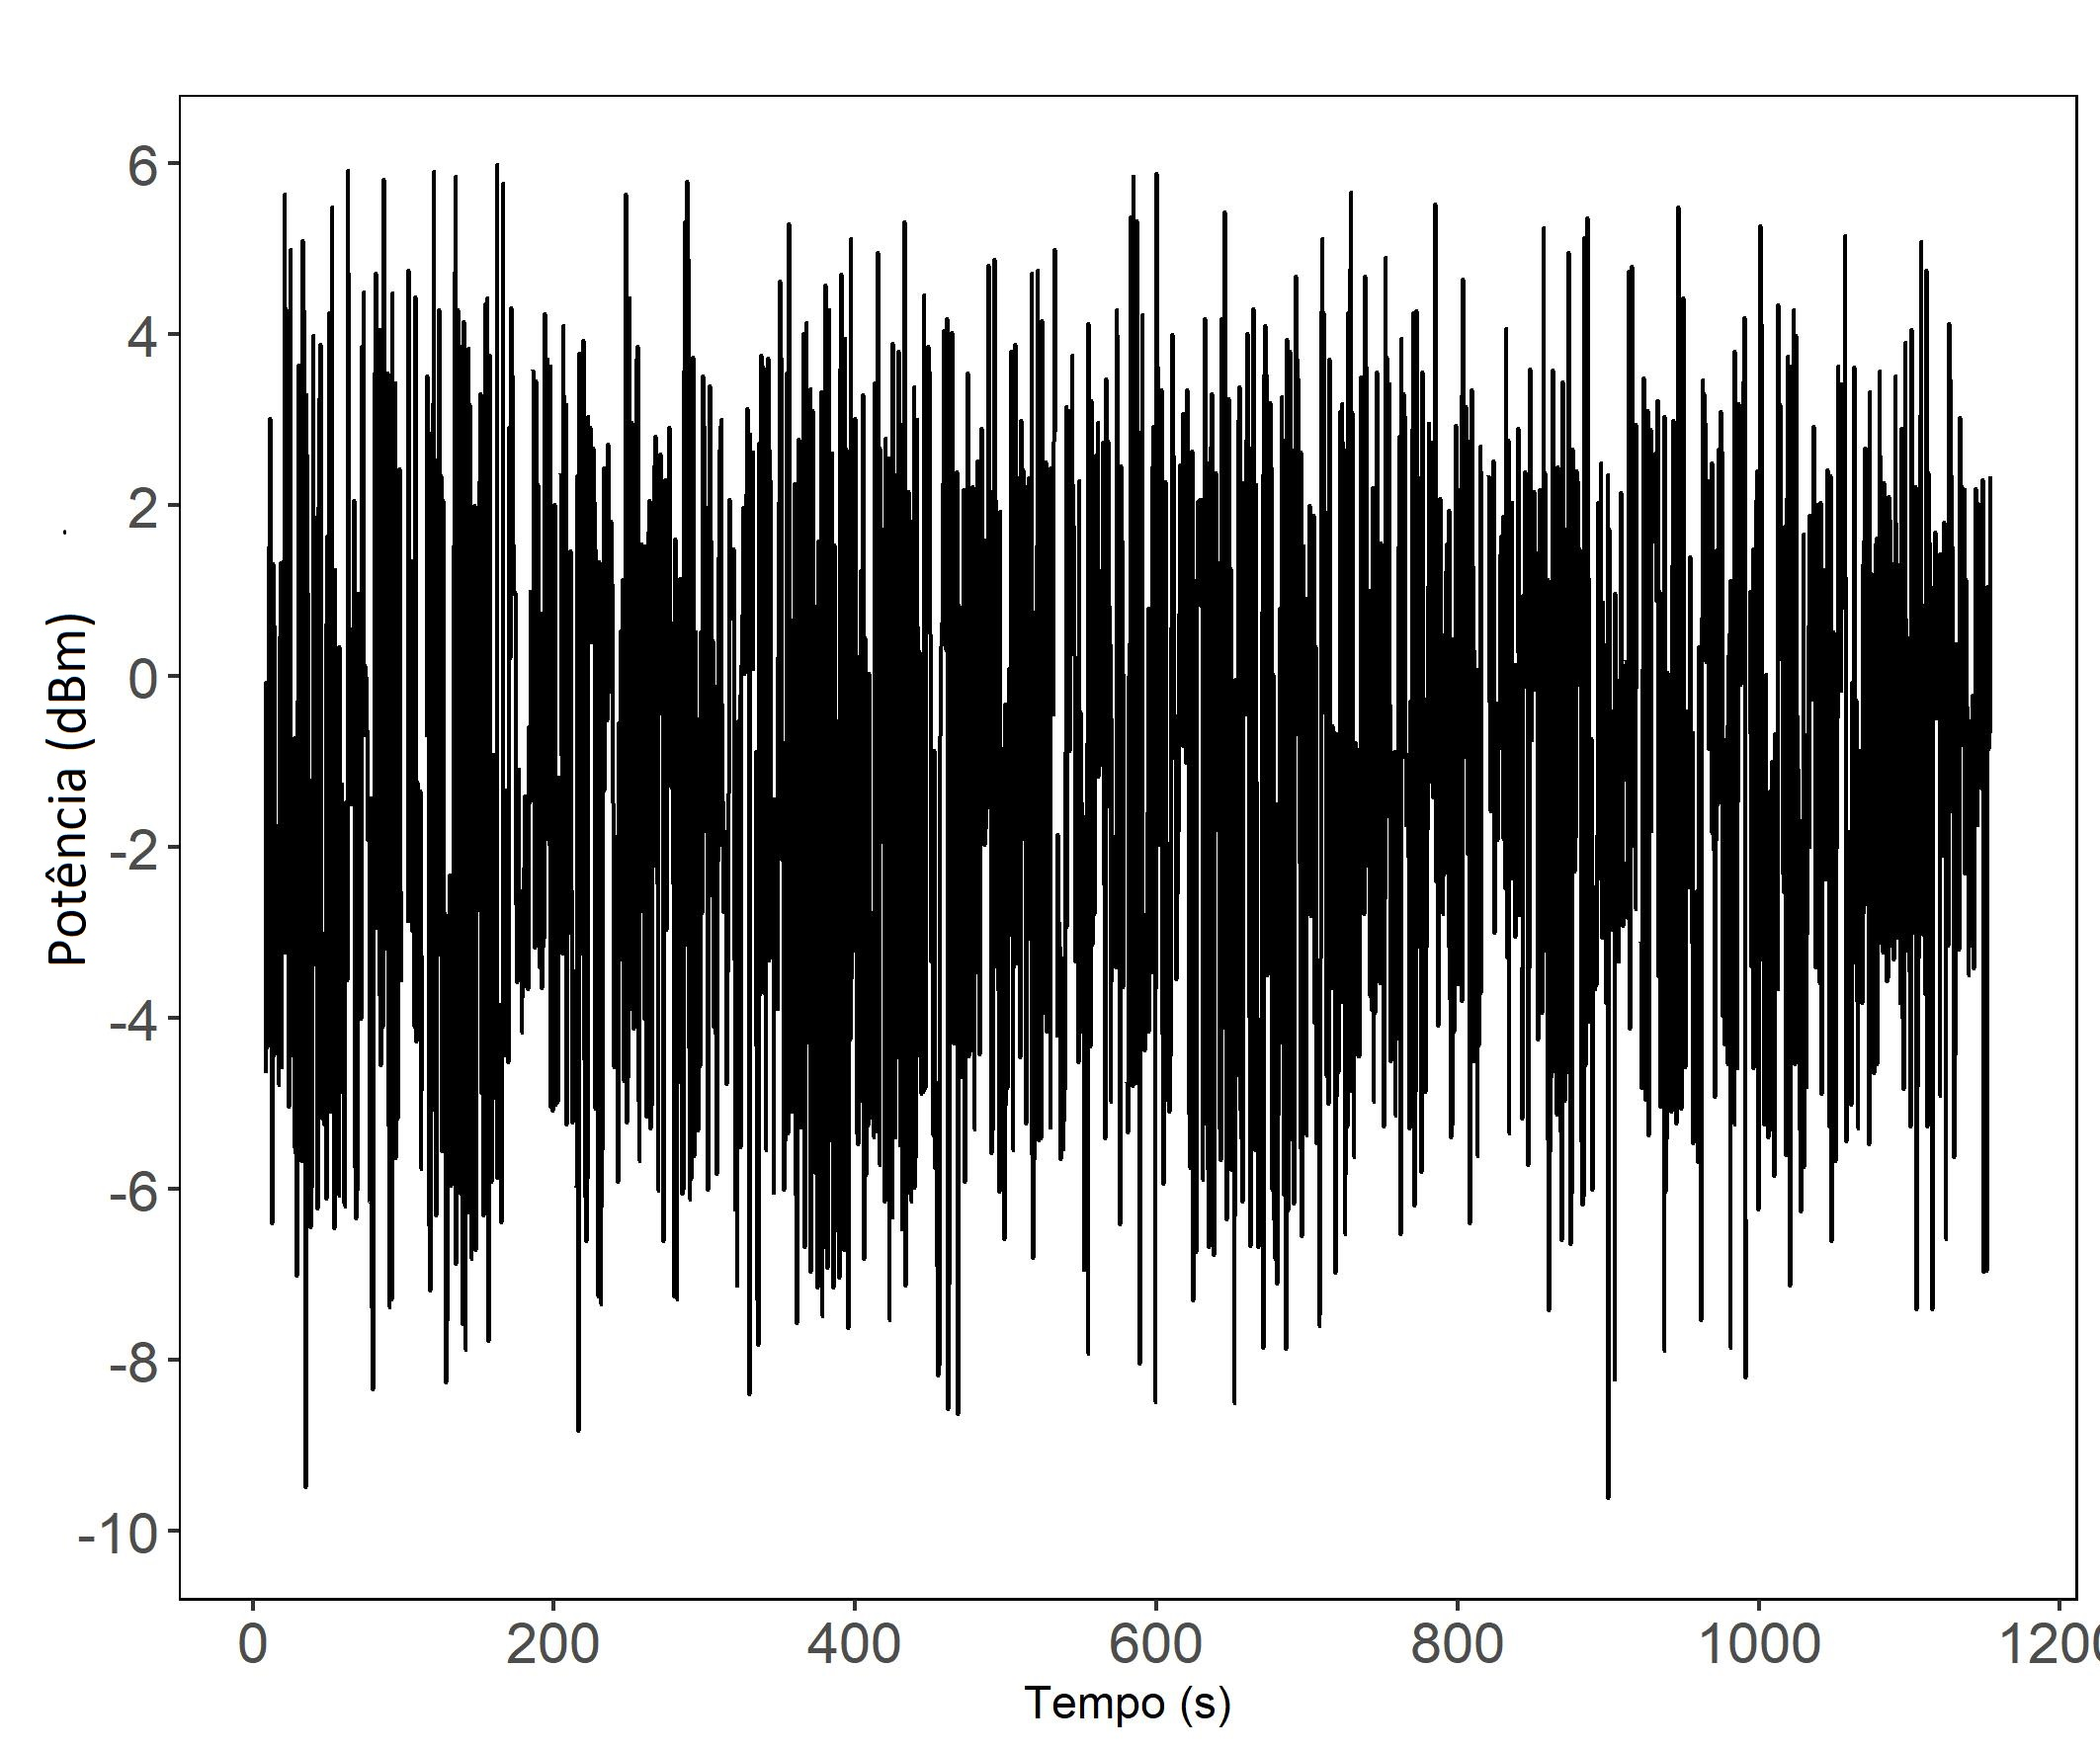
\includegraphics[height=0.37\columnwidth]{dia1alto.jpeg}}
    ~
%    \subfigure[\label{fig:ptrx_omni_baixo} Exemplo dia 1, baixo fluxo .]{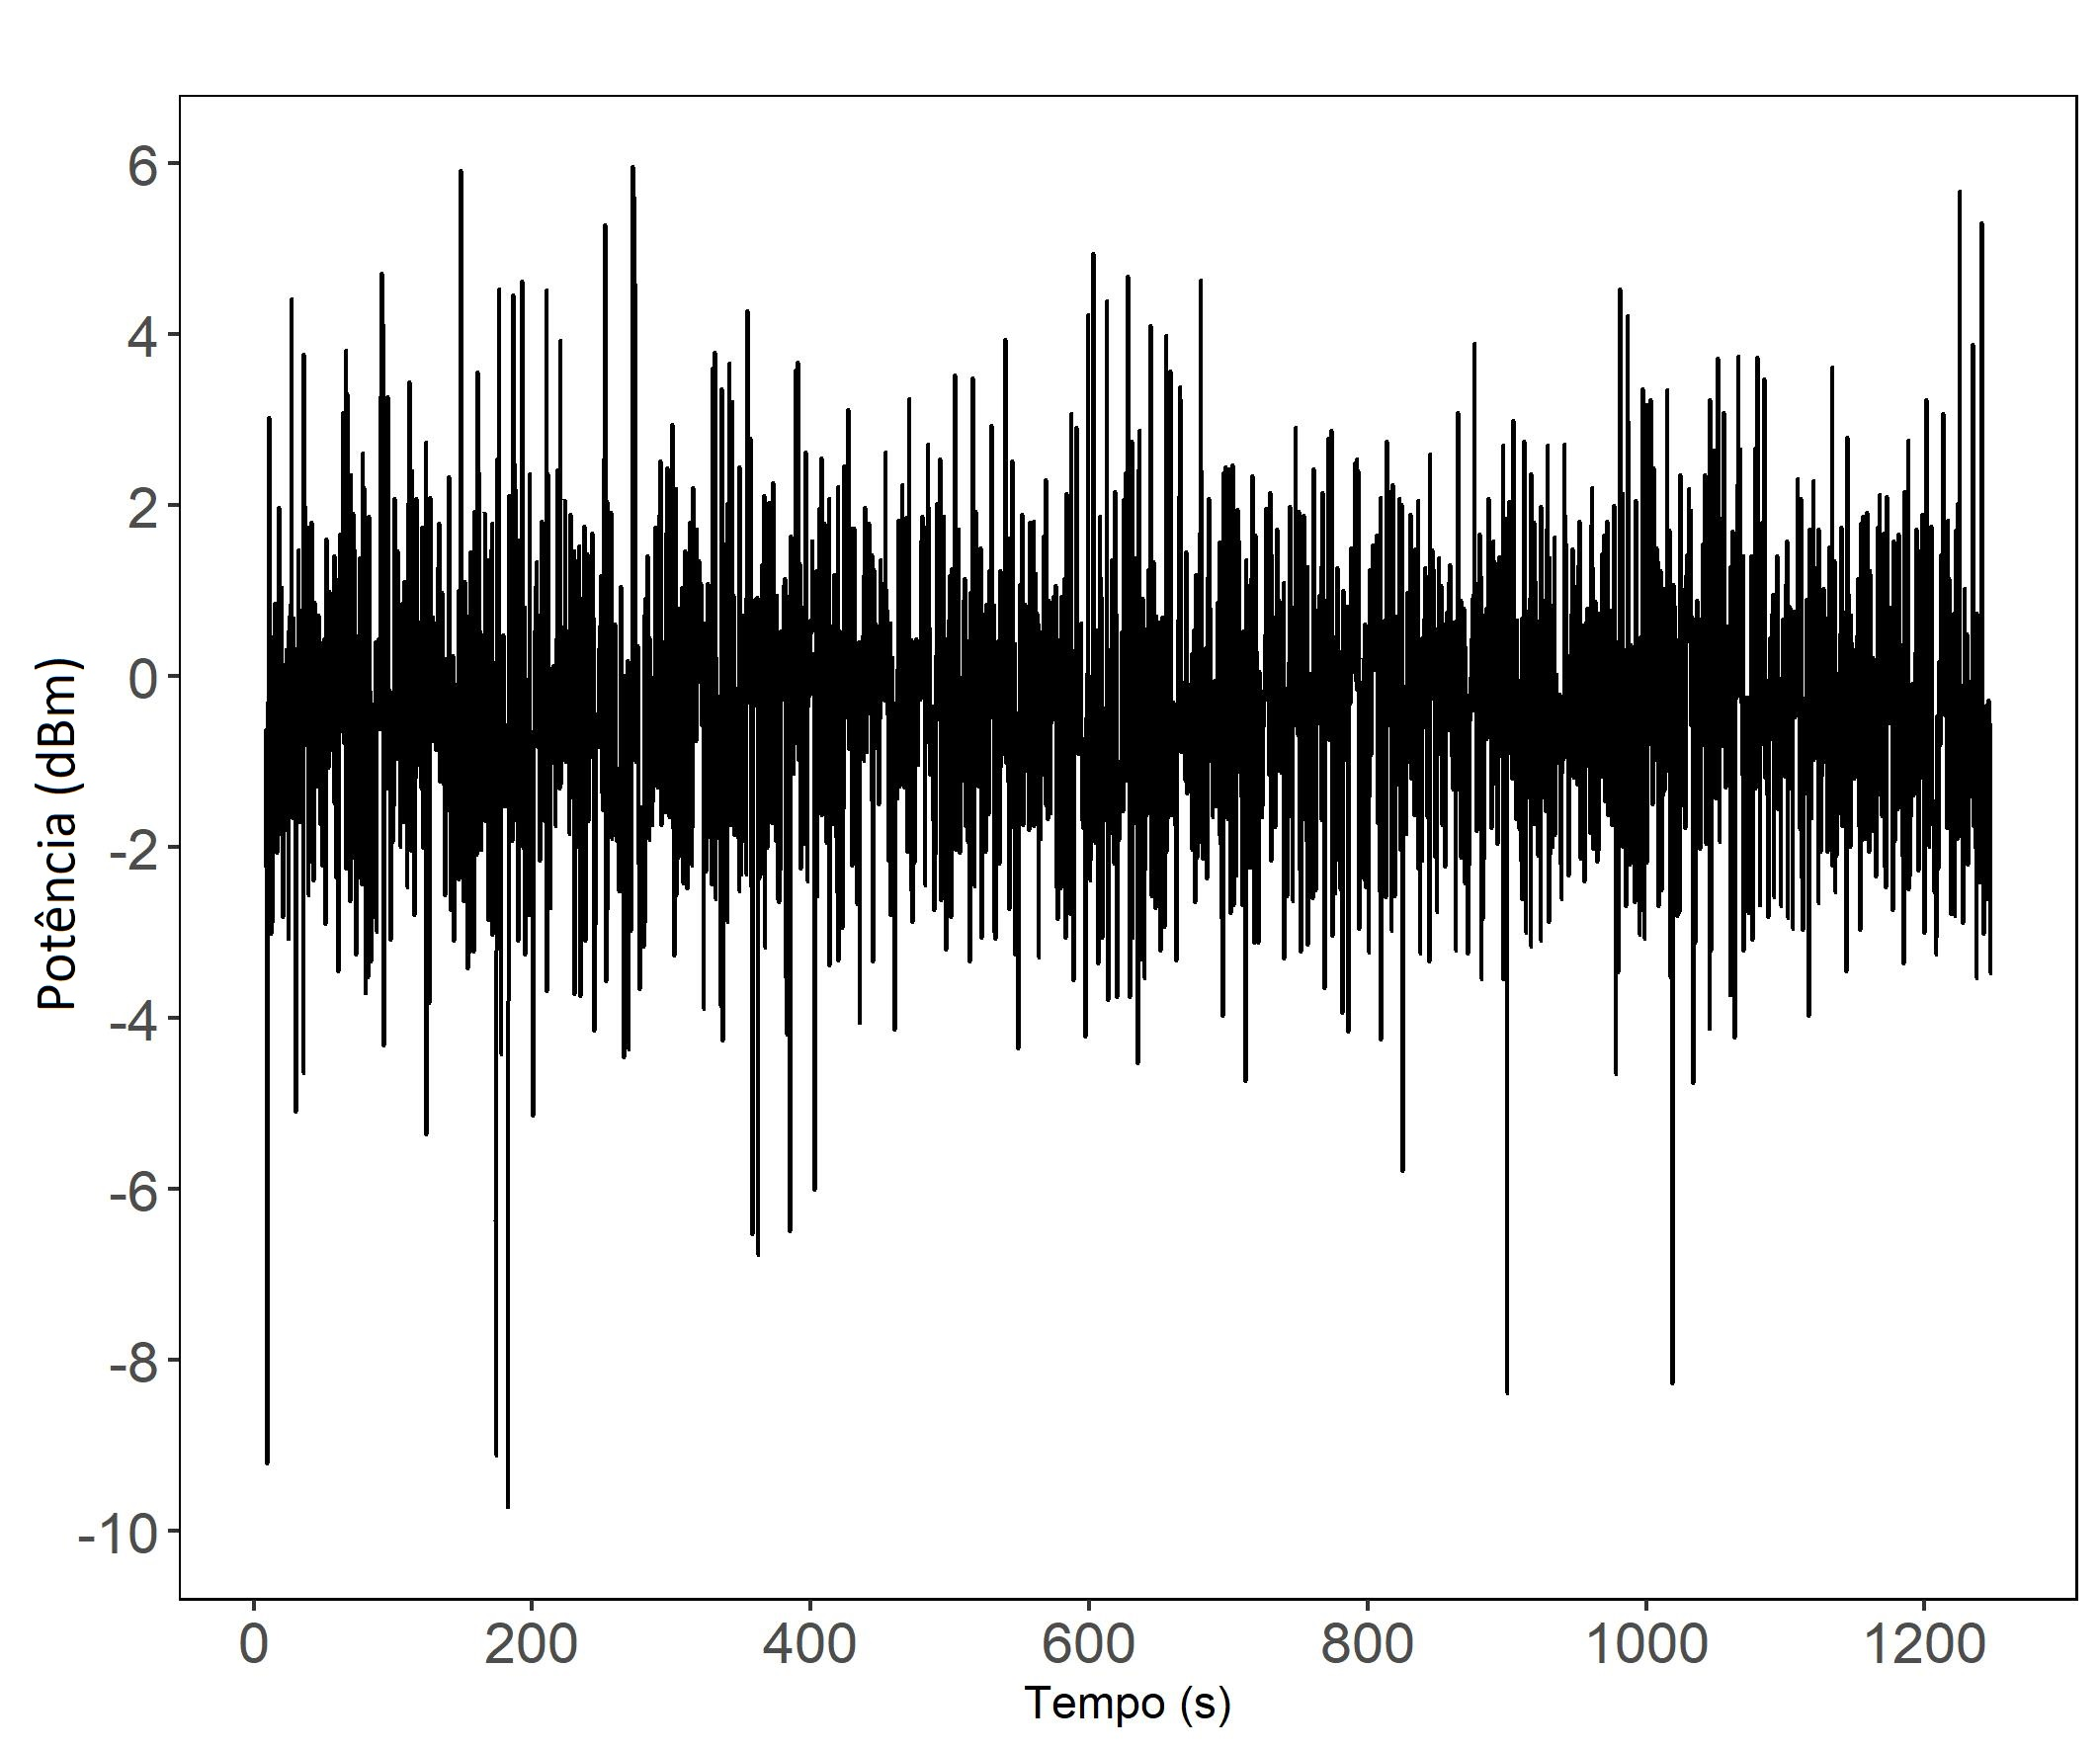
\includegraphics[height=0.37\columnwidth]{dia1baixo.jpeg}}
    %
%    \subfigure[\label{fig:ptrx_micro_alto} Exemplo dia 2, alto fluxo.]{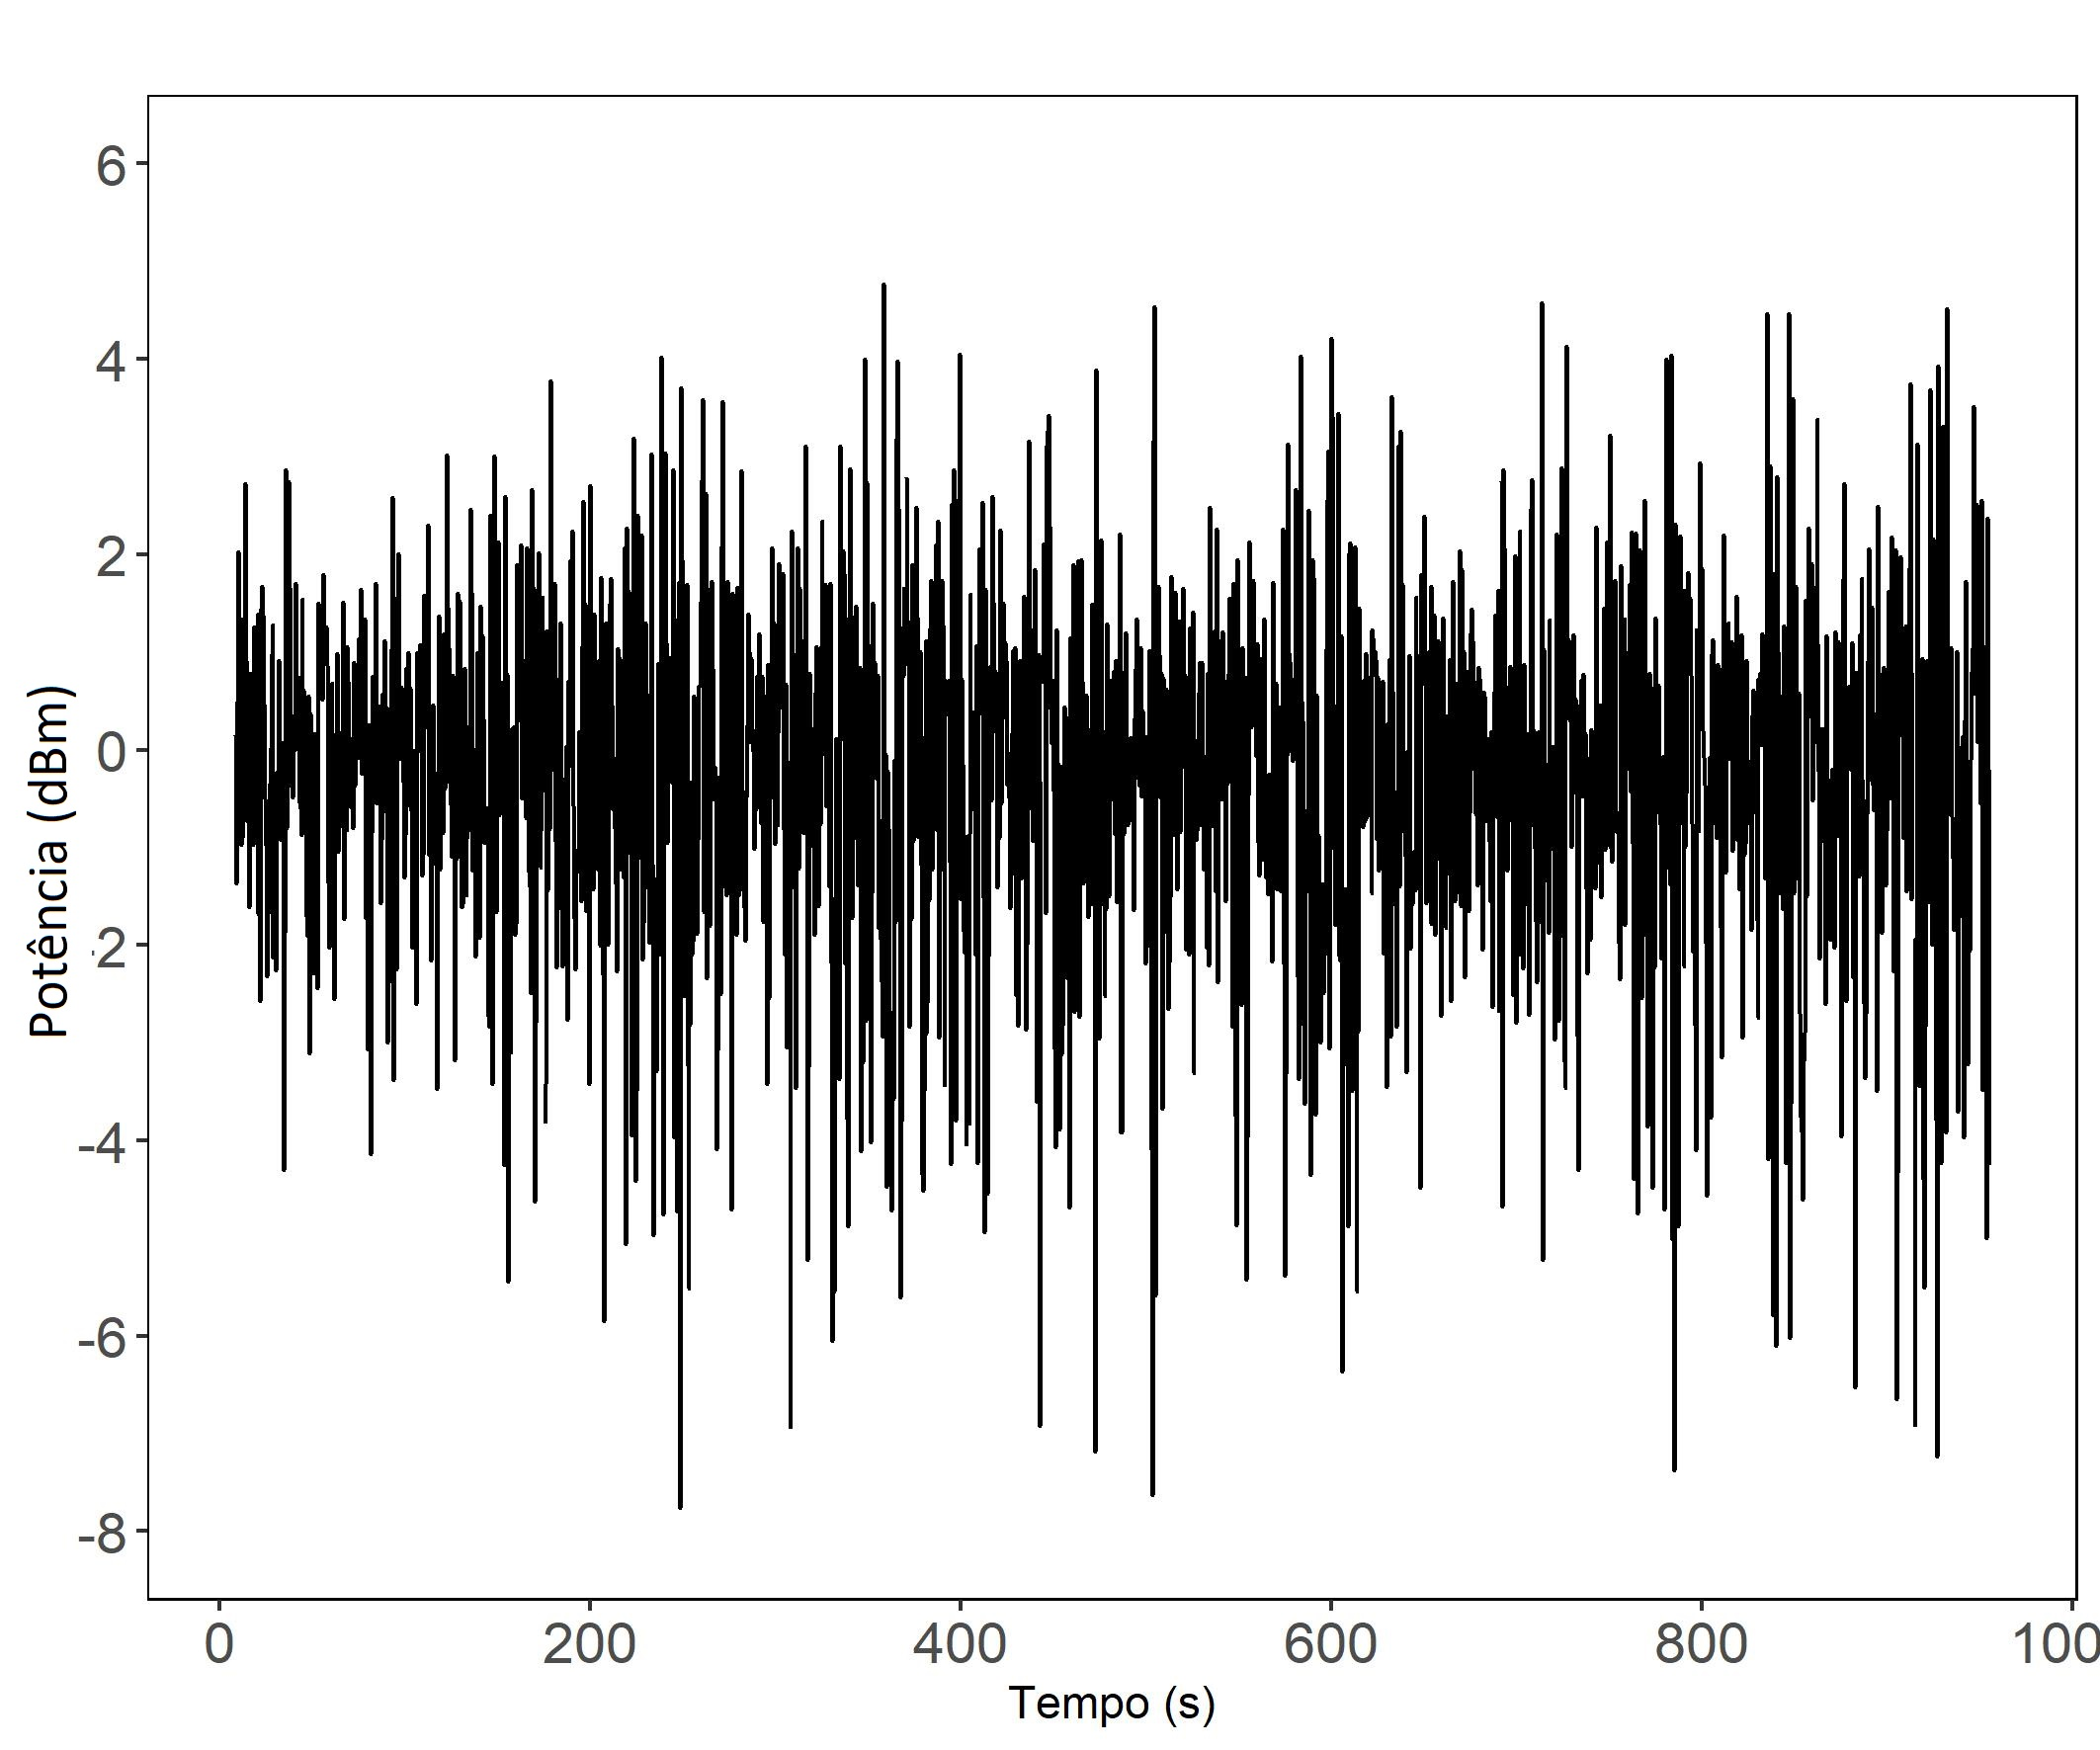
\includegraphics[height=0.37\columnwidth]{dia2alto.jpeg}}
    ~
%    \subfigure[\label{fig:ptrx_micro_baixo} Exemplo dia 2, baixo fluxo.]{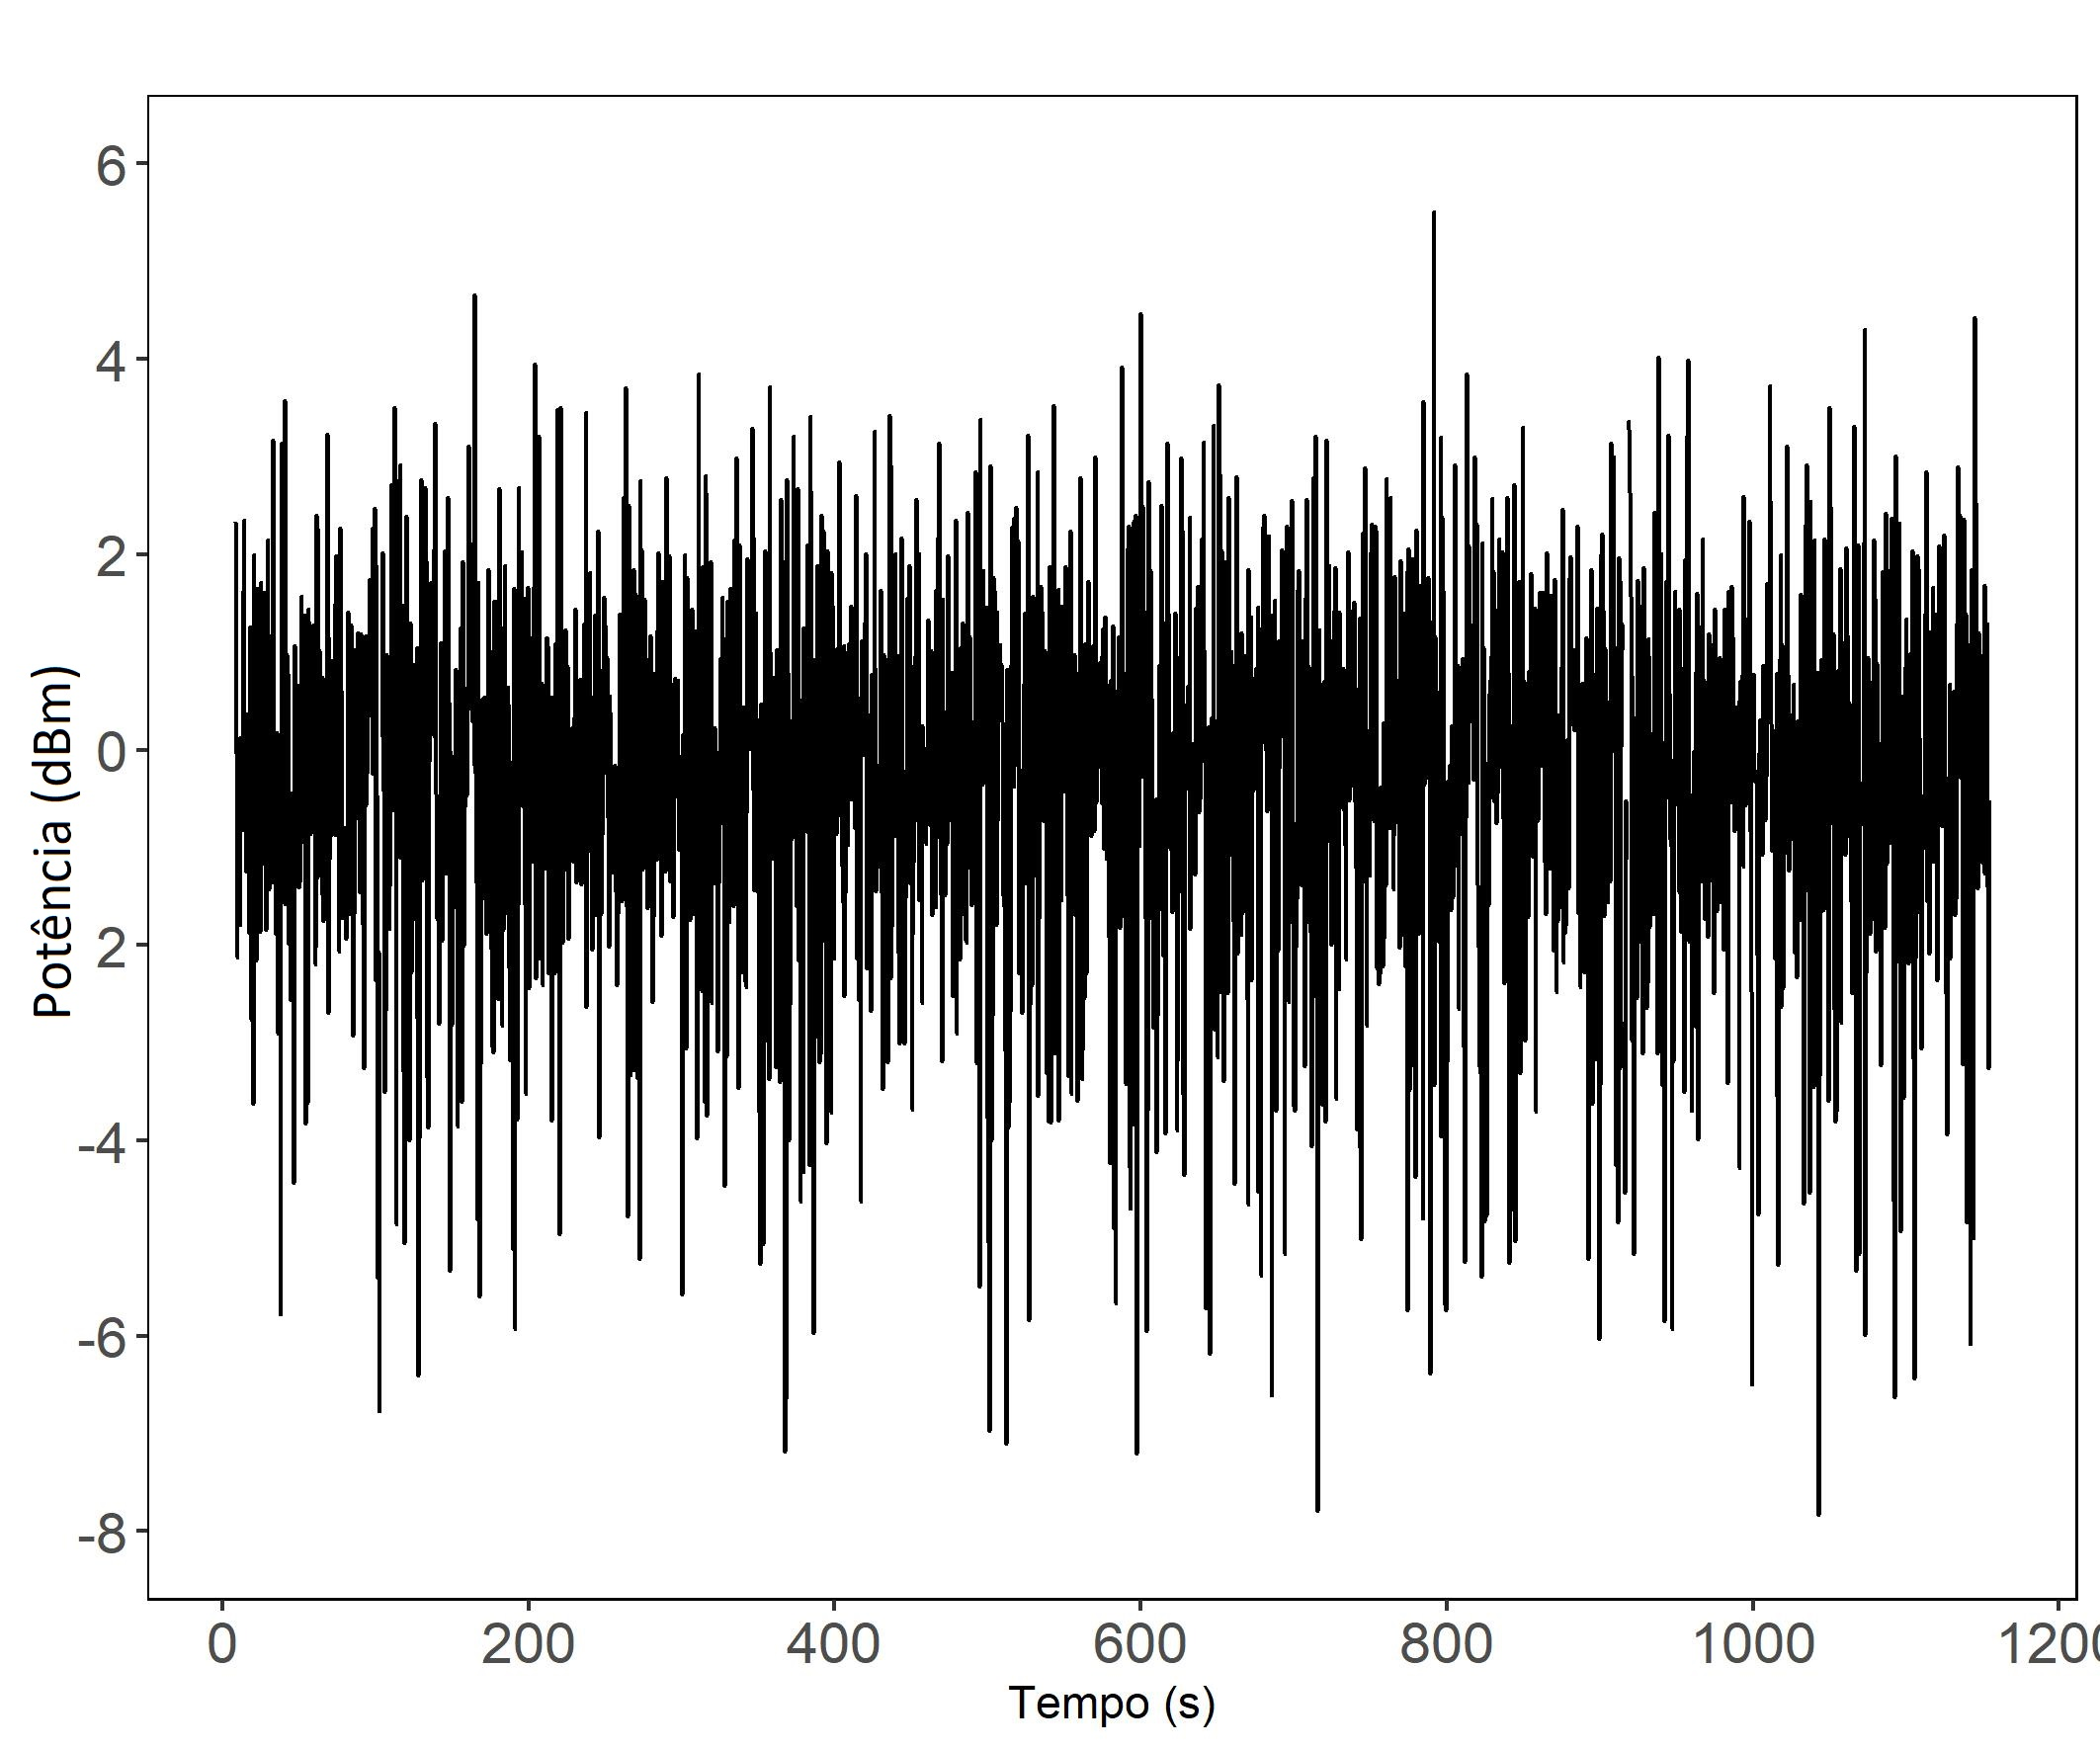
\includegraphics[height=0.37\columnwidth]{dia2baixo.jpeg}}
    %
%    \caption{\label{fig:ptrx} Exemplo de resultados das medições.}
%\end{figure}

%Pode-se verificar, comparando as Figuras~\ref{fig:ptrx_omni_alto} e \ref{fig:ptrx_omni_baixo}, uma maior variabilidade do sinal recebido em uma situação com fluxo alto  em relação à condição de menor fluxo. Do mesmo modo, comparando as Figuras~\ref{fig:ptrx_micro_alto} e \ref{fig:ptrx_micro_baixo}, é possível ver que o sinal referente à situação com maior fluxo apresenta uma variabilidade maior. Porém essa diferença é bem menos acentuada, devido à ... 



%Finalmente, foram calculadas as estatísticas de segunda ordem (teóricas e empíricas). Ambas TCN e DMD resultaram em estimativas de $\hat{f}_m$ similares, como mostrado na Figura~\ref{fig:TCN}. 

%
%\begin{figure}[ht]
%    \centering
%    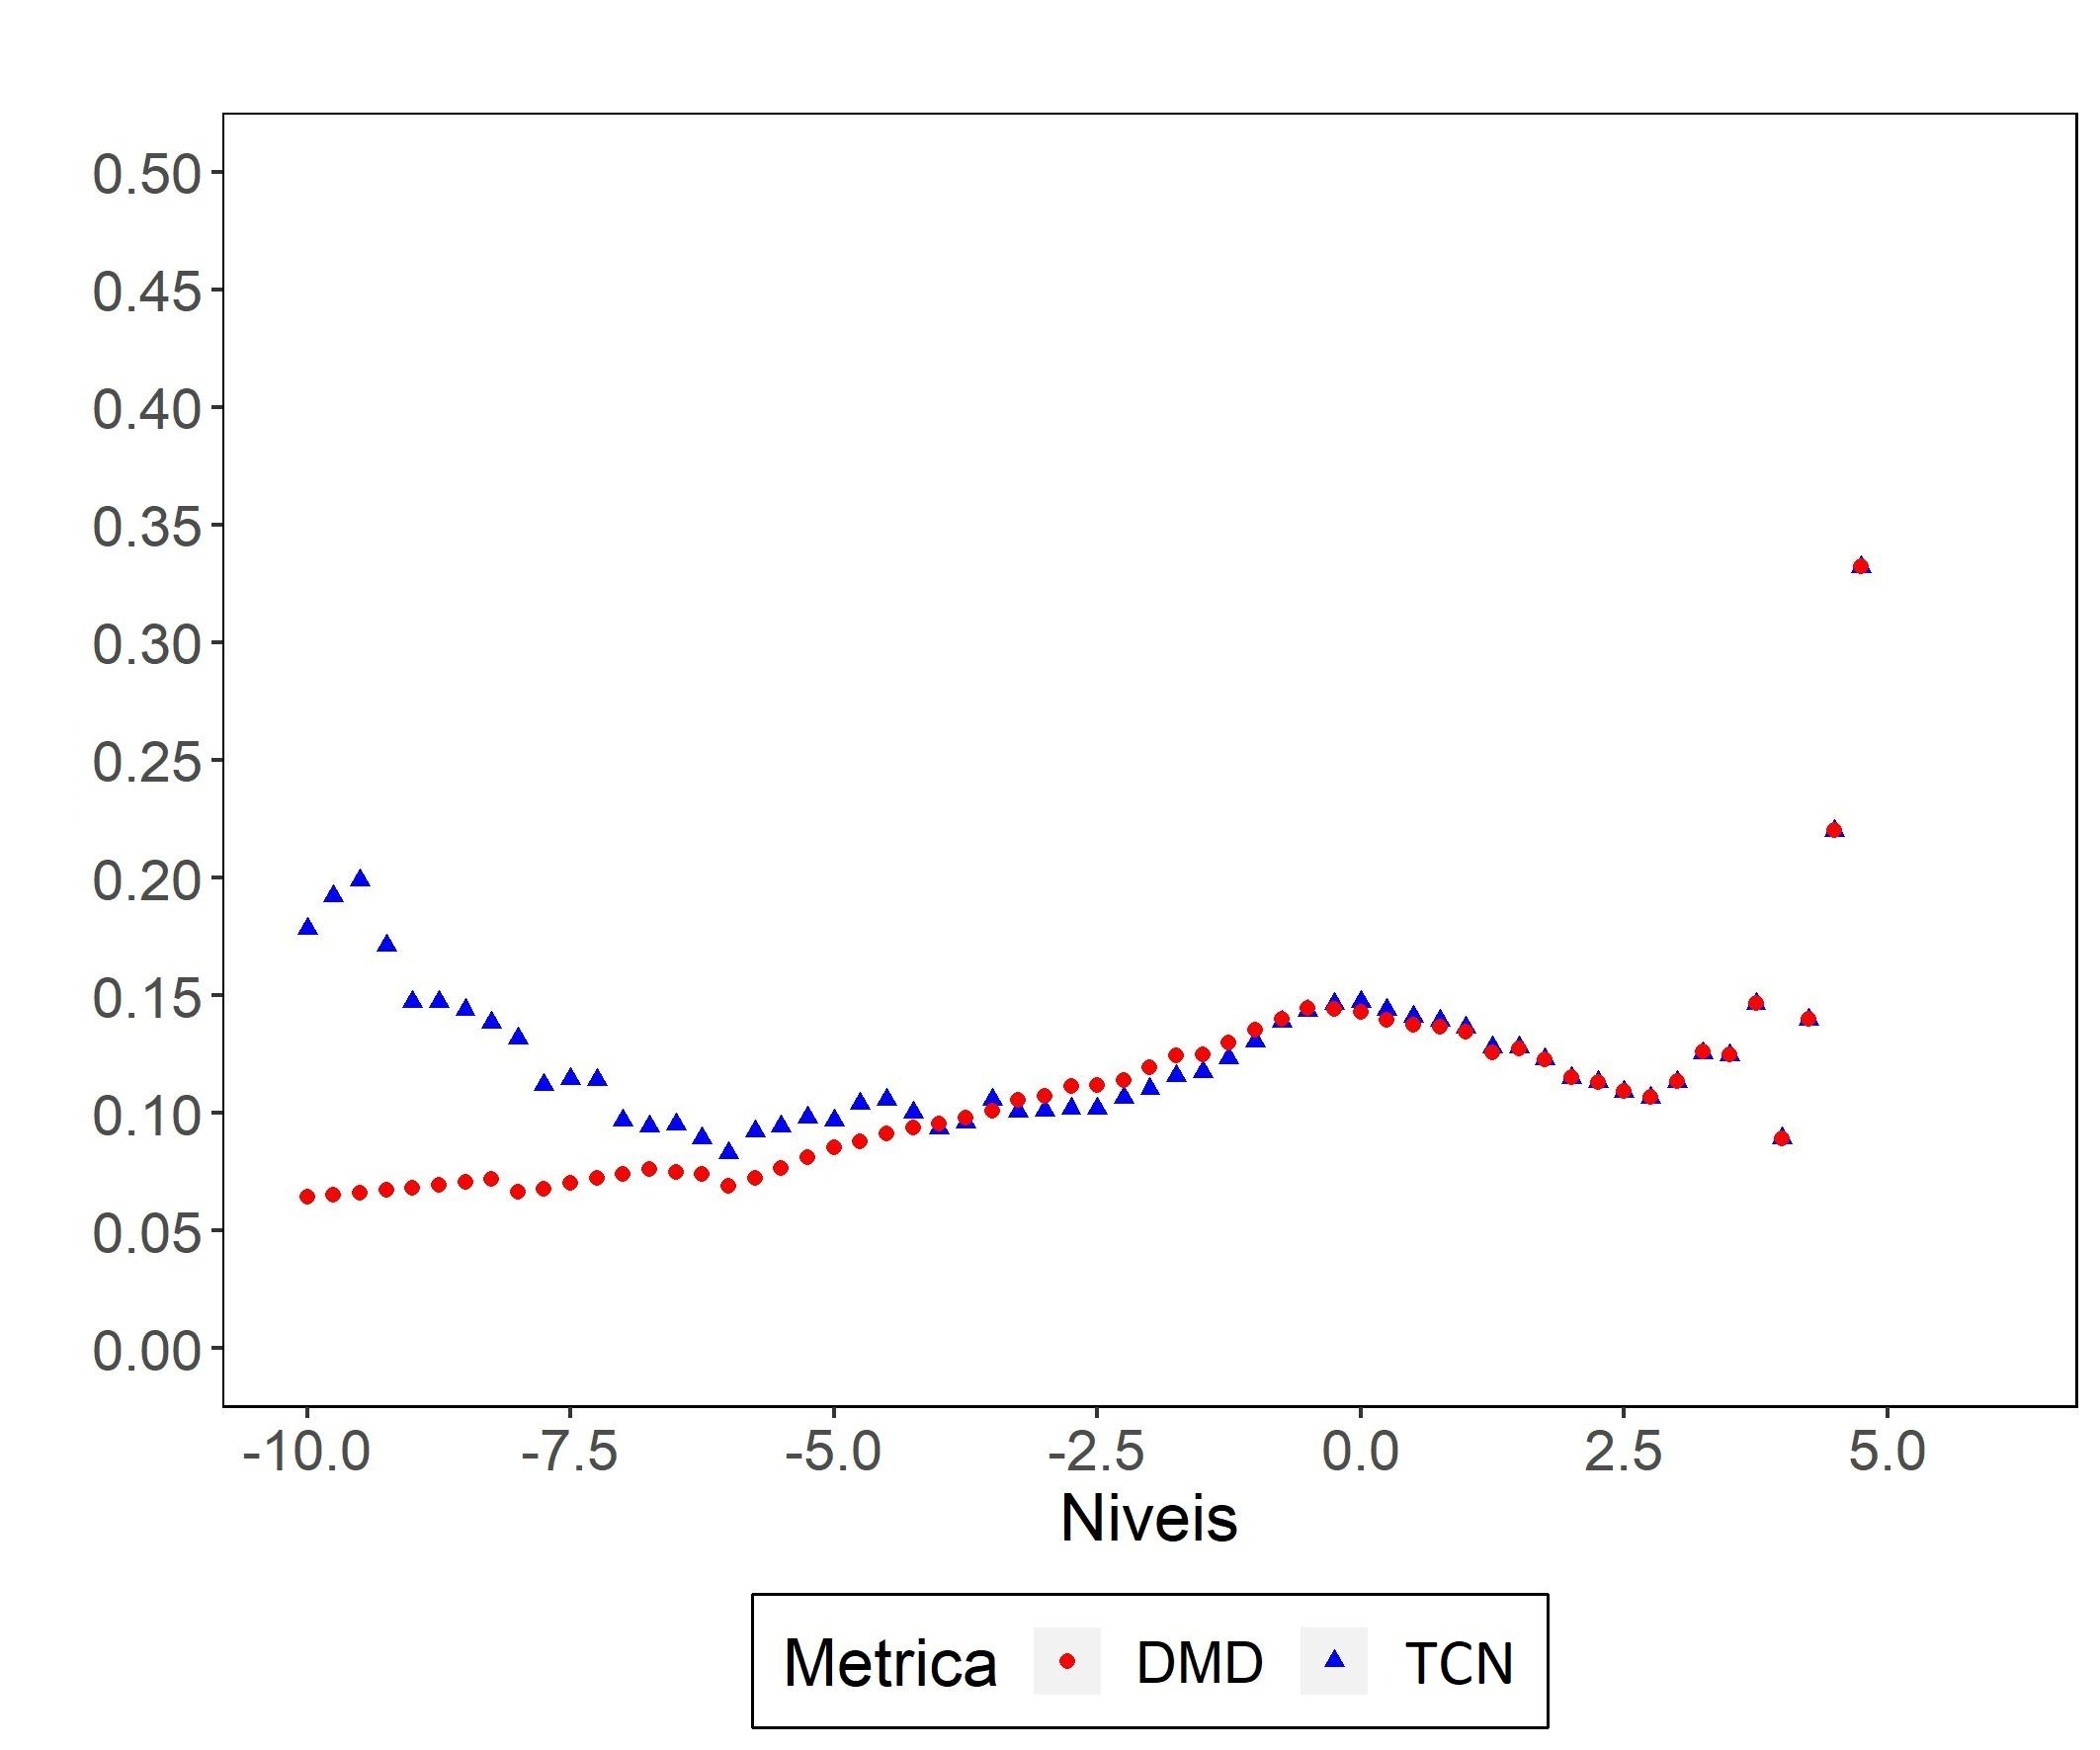
\includegraphics[height=0.5\columnwidth]{fm.jpeg}
%    \label{fig:TCN}
%    \caption{Exemplo de gráfico com resultados.}
%\end{figure}
%

%Na Figura~\ref{fig:TCN}, observa-se que o gráfico da TCN é mais esparso que o gráfico da DMD. Isso reforça a conclusão que as amostras colhidas na condição de baixo fluxo  apresentam uma menor variabilidade em relação à condição de alto fluxo. 

\section{Apresentação e Discussão dos Resultados}
\subsection {Características da amostra e estudo de independência}
Após a aplicação dos métodos apropriados para se tirar as primeiras conclusões a respeito dos dados, obteve-se a tabela 1 que resume a amostra selecionada, a qual se refere ao consumo energético do mês de março, às 4h, durante os 13 anos.

\begin{table}[!htb]
\centering
\caption{\textsc{Estatísticas Descritivas do Consumo (Mês 03).}}
\label{tab:estatisticas}
\begin{tabular}{l r}
\hline\hline
\textbf{Métrica} & \textbf{Valor} \\
\hline
Tamanho da amostra         & 403 \\
Média (MW)                 & 13758,0223 \\
Mediana (MW)               & 13737,0000 \\
Moda (MW)                  & 12884,0000 \\
Mínimo (MW)                & 9917,0000 \\
Máximo (MW)                & 19240,0000 \\
Amplitude (MW)             & 9323,0000 \\
Desvio-padrão (amostral) [MW] & 1700,2358 \\
Variância da amostra [MW\(^2\)] & 2890801,9174 \\
\textbf{Coeficiente de Variação} & \textbf{0,1236} \\
Coeficiente de Assimetria  & 0,1954 \\
\hline\hline
\end{tabular}
\end{table}

A análise descritiva das 403 observações, indica consumo médio de 13.758 MW, mediana de 13.737 MW e desvio‑padrão amostral de aproximadamente 1.700 MW, resultando em coeficiente de variação (CV) de 12,36\%. Sabe-se que CVs menores que 15\% apontam para uma dispersão moderada em torno da média, sugerindo relativa estabilidade do consumo no período analisado e adequação da amostra selecionada.

O \emph{boxplot} apresentado na Figura 1 resume a distribuição do consumo no mês analisado, evidenciando a presença de um \emph{outlier} moderado no valor de 19.240 MW. A mediana do consumo é de 13.737 MW, com limites inferior e superior (Li e Ls) de 8.440,25 MW e 19.118,25 MW, respectivamente. O primeiro quartil (Q1) situa-se em 12.444,50 MW e o terceiro quartil (Q3) em 15.114,00 MW, indicando que 50\% dos dados estão concentrados nesse intervalo. Pela não evidência de erros de coleta e por não se tratar de um valor extremo, optou-se por não retirar este valor do conjunto e seguir com as análises.

\begin{figure}[!htb]
    \centering
    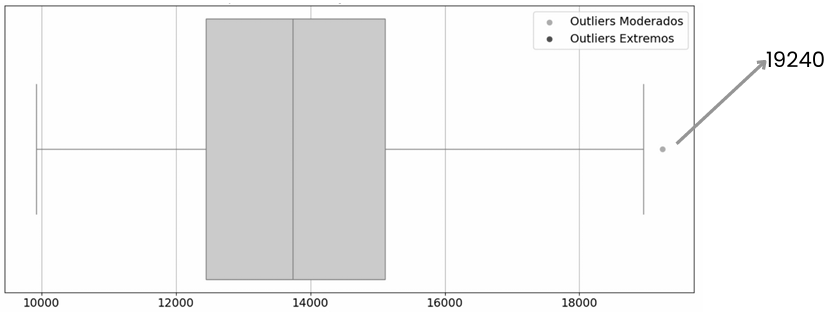
\includegraphics[width=0.48\textwidth]{Boxpplot_pb.png}
    \caption{Boxplot modificado e \emph{outlier} moderados}
    \label{fig:boxplot_consumo}
\end{figure}

O histograma mostrado na figura 2 (método de Rice), em conjunto com o teste de Kolmogorov–Smirnov (valor‑p = 0,201; alfa = 0,05), mostram que a distribuição candidata, a normal, não deve ser rejeitada, o que reforça a adequação do ajuste probabilístico. 

\begin{figure}[!htb]
    \centering
    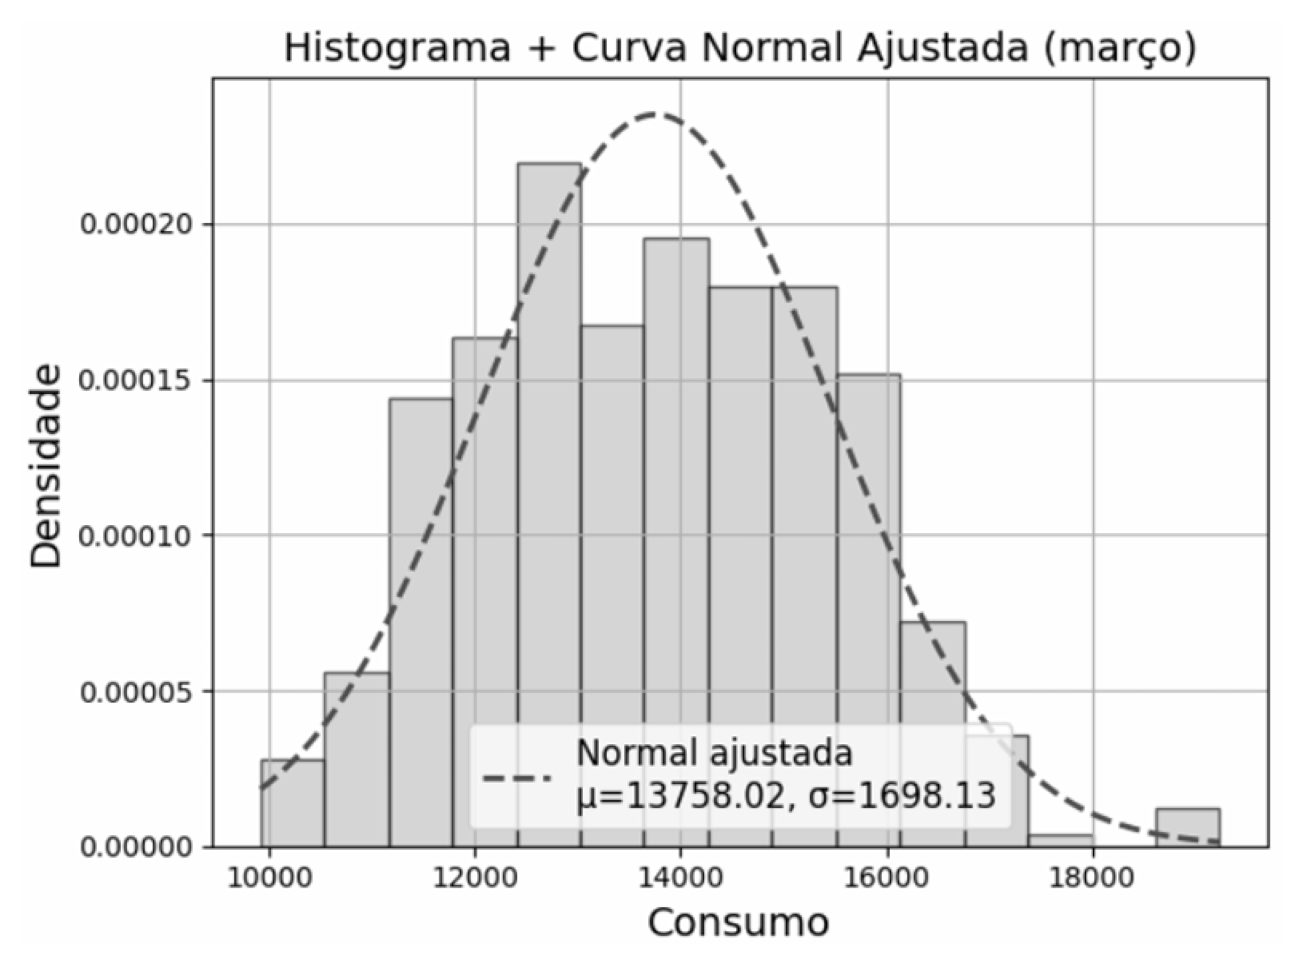
\includegraphics[width=0.48\textwidth]{histo.png}
    \caption{ Histograma da amostra selecionada}
    \label{fig:histo.png}
\end{figure}


Por outro lado, o teste de Ljung–Box com defasagem 10 apresentou valor‑p extremamente baixo (aproximadamente $9,41 \times 10^{-87}$), rejeitando a hipótese de independência entre as observações e evidenciando autocorrelação. Assim, embora a distribuição ajustada represente bem a forma geral dos dados, a dependência temporal do consumo desaconselha o uso de um modelo puramente i.i.d., motivando a adoção de abordagens por séries temporais.

\subsection {Tratamento da amotra como séries temporais}
A segunda etapa da modelagem consistiu na análise da série temporal referente ao mês de novembro de 2016, utilizada como base para a calibração do modelo. O teste de estacionariedade de Dickey–Fuller Aumentado (ADF) apresentou estatística de $-1{,}914$, com valor-p igual a $0{,}326$, superior ao valor crítico de 5\% ($-2{,}866$). Dessa forma, a série foi caracterizada como não estacionária. 

\begin{figure}[!htb]
    \centering
    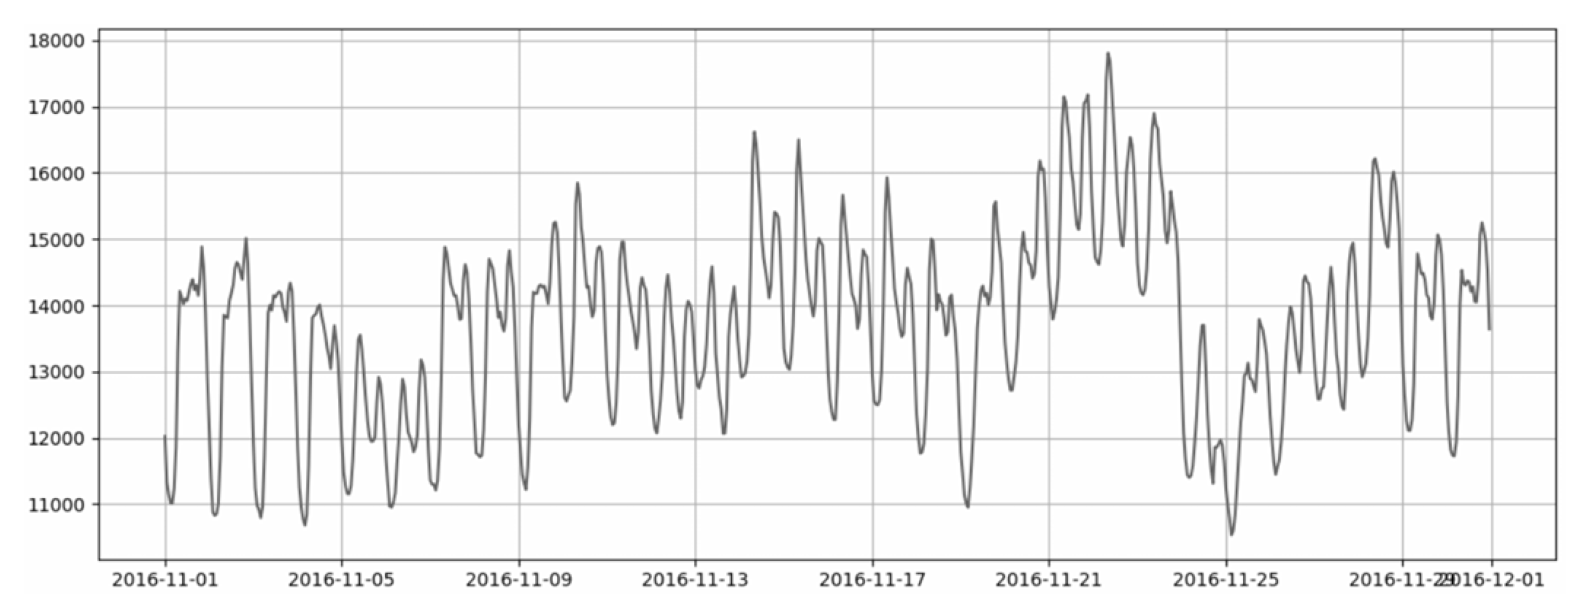
\includegraphics[width=0.48\textwidth]{naoesta.png}
    \caption{ Padrão não estacionário da amostra}
    \label{fig:naoesta.png}
\end{figure}


Após a diferenciação de primeira ordem ($d=1$), a estatística ADF passou a $-11{,}94$, com valor-p igual a $0$, confirmando a estacionariedade da série diferenciada. A figura 4 mostra os valores variando aleatoriamente em torno de uma média nula.

\begin{figure}[!htb]
    \centering
    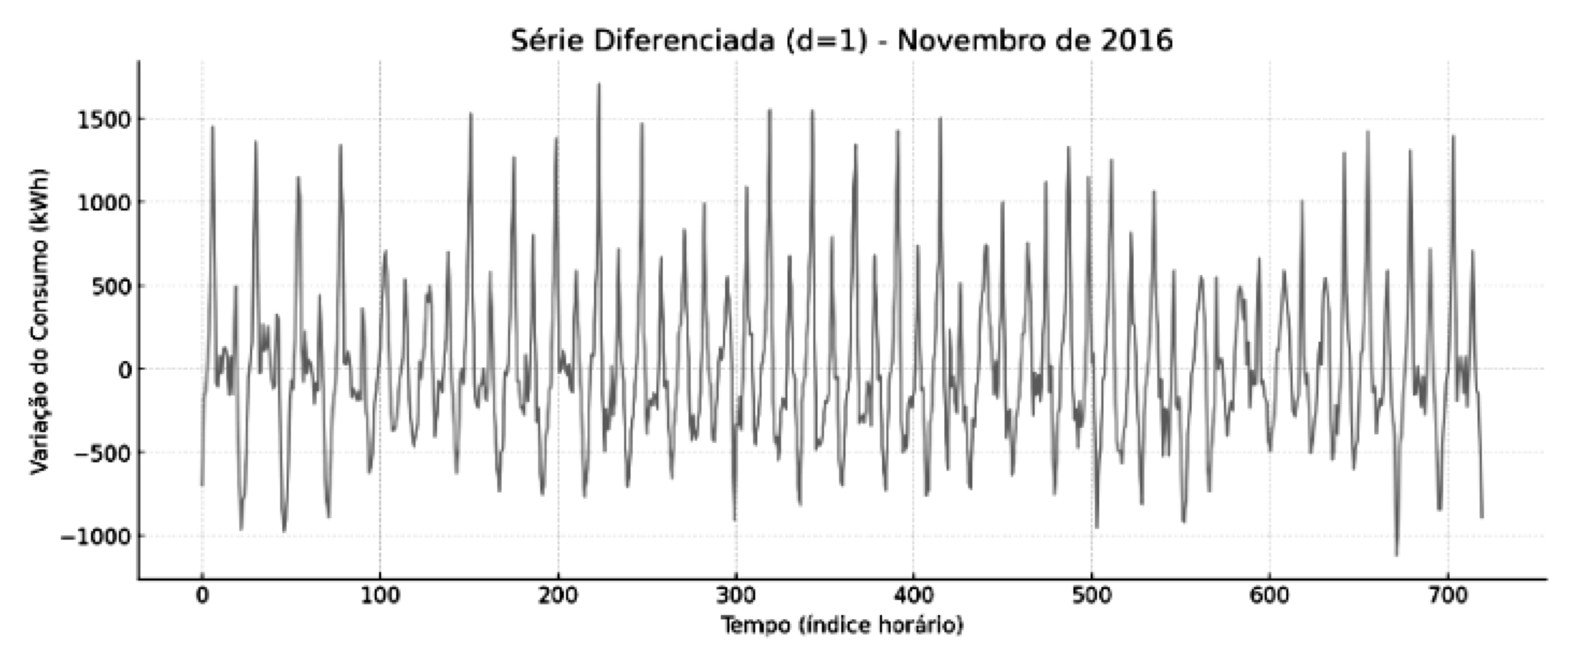
\includegraphics[width=0.48\textwidth]{esta.png}
    \caption{ Padrão estacionário da amostra após a aplicação de d = 1}
    \label{fig:esta.png}
\end{figure}

A análise das funções de autocorrelação (ACF) e autocorrelação parcial (PACF) indicou a presença de um comportamento típico de processos autorregressivos e de médias móveis de primeira ordem. Assim, foi proposto o modelo ARIMA$(1,1,1)$ para representação da série temporal de consumo de energia elétrica e o modelo de diferenciação expresso na equação 8.

\begin{equation}
\Delta Y_{t} = 0{,}5186 \cdot \Delta Y_{t-1} + \varepsilon_{t} + 0{,}3825 \cdot \varepsilon_{t-1}
\end{equation}


O modelo ARIMA$(1,1,1)$ foi ajustado inicialmente aos dados de novembro de 2016 (\emph{in-sample}), apresentando um erro percentual absoluto médio (MAPE) de 1,73\% na amostra de teste, valor obtido a partir da previsão realizada para o período do dia 01/12/2016 às 0:00h onde o valor previsto de 12.974,19 MW, mostrando boa proximidade com o valor real de 12.949 MW. 

Na sequência, o modelo foi aplicado aos dados de novembro de 2017, a fim de verificar sua robustez. Nesse cenário, o MAPE obtido foi de 1,42\%, ao se realizar uma previsão para 01/12/2017 - 0:00h, onde o valor previsto consumido foi de 13.926,16 MW e o real de 13.483 MW.

Apesar do bom desempenho em termos de acurácia, a análise dos resíduos (\emph{in-sample} e \emph{out-of-sample}) revelou a presença de autocorrelação significativa. O teste de Ljung–Box aplicado aos resíduos resultou em estatísticas de 111,51 (p-valor $\approx 2,64\times10^{-19}$) para novembro de 2016 e de 137,94 (p-valor $\approx 1,11\times10^{-24}$) para novembro de 2017, rejeitando a hipótese nula de ausência de autocorrelação. Esses resultados indicam que, embora o ARIMA$(1,1,1)$ forneça previsões satisfatórias, ainda há estrutura remanescente nos resíduos que não é capturada pelo modelo.

Em síntese, os objetivos propostos foram atingidos: o modelo ARIMA$(1,1,1)$ apresentou baixo erro de previsão. Contudo, a presença de autocorrelação nos resíduos sugere a necessidade de investigações adicionais, incluindo a comparação com outros modelos, tais como redes neurais artificiais ou modelos híbridos, que poderão capturar de forma mais completa a dinâmica da série temporal de consumo de energia elétrica.



\section{Conclusões}
\label{sec_conclusoes}

O objtivo principal deste trabalho foi atingido, e os resultados obtidos demonstraram que o modelo ARIMA(1,1,1) apresentou bom desempenho para previsão do consumo elétrico, tanto no ajuste \emph{in-sample} (novembro de 2016) quanto em um período posterior (novembro de 2017). O erro percentual absoluto médio (MAPE) foi de 1,73\% e 1,42\%, respectivamente, o que evidencia a capacidade do modelo em gerar estimativas precisas. Entretanto, os testes de Ljung--Box aplicados aos resíduos revelaram a presença de autocorrelação significativa, indicando que ainda há padrões na série que não foram plenamente capturados pelo modelo.

Como trabalhos futuros, sugere-se a investigação de modelos mais robustos, tais como métodos híbridos que combinem abordagens estocásticas clássicas com técnicas de aprendizado de máquina. Em especial, o uso de redes neurais recorrentes (RNN) ou modelos baseados em \textit{Long Short-Term Memory} (LSTM) pode permitir capturar de forma mais eficiente as dependências de longo prazo. Além disso, recomenda-se avaliar a aplicação da metodologia em outros contextos regionais ou em séries mais recentes, visando generalizar os achados e contribuir para a melhoria dos sistemas de previsão de demanda energética.

%Nesta Seção, deve-se descrever rapidamente a motivação do problema e resumir o que foi feito no trabalho. 

%Outro parágrafo é acrescentado para descrever os principais resultados obtidos com as análises.

%Opcionalmente, pode-se incluir mais um parágrafo descrevendo possíveis trabalhos futuros.
%\section*{Agradecimentos}
%Este trabalho foi realizado com apoio da Coordenação de Aperfeiçoamento de Pessoal de Nível Superior - Brasil (CAPES) - Código de Financiamento 001.
\bibliographystyle{IEEEtran}
\bibliography{referencias}
%\newpage
\begin{IEEEbiography}[{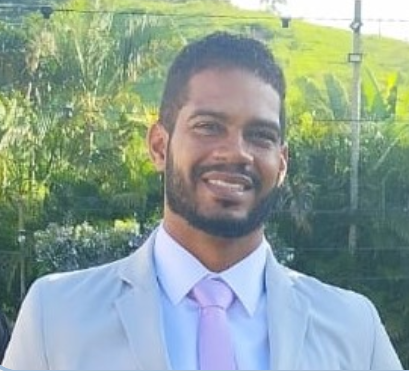
\includegraphics[width=1in,clip,keepaspectratio]{foto.png}}]{\textbf{Everton Costa Santos}} 
Bacharel em Engenharia de Produção e Sistemas e Mestre em Modelagem Computacional em Ciência e Tecnologia, ambos pela Universidade Estadual de Santa Cruz - UESC. Atua como docente no Instituto de Ciência, Engenharia e Tecnologia - ICET - na Universidade Federal dos Vales do Jequitinhonha e Mucuri - UFVJM - Campus do Mucuri. Possui interesse nas áreas Engenharia do Produto e Modelagem e Simulação de Processos Produtivos.  
\end{IEEEbiography}

\end{document}
